%% Theory of Computing
%% File: v016a013.tex
%% Publication date: November 9, 2020
%% Authors: Ankit Garg, Mika Goos, Pritish Kamath, and Dmitry Sokolov
%
%
%
%

%

%
%

%
%
%
%
%
%
%
%
%
%
%
%
%
%
%
%
%
%
%
%
%
%
%
%

%

\documentclass{toc}

%
\usepackage{mathtools,thmtools}
%
%
\usepackage{lpic,bm,xspace}

\usepackage{algorithmicx,algorithm}
\usepackage[noend]{algpseudocode}

\usepackage{caption}

\usepackage{dsfont}
\usepackage[english]{babel}
\addto\extrasenglish{\def\sectionautorefname{Section}}
\addto\extrasenglish{\def\subsectionautorefname{Section}}
%
%

\usepackage{enumitem}
\setlist[itemize]{noitemsep,label=$-$}
\setlist[enumerate]{noitemsep}


\usepackage{tikz}
\usepackage[framemethod=tikz]{mdframed}
\mdfsetup{
	roundcorner=4pt,
	nobreak=true,
	linewidth=.5,
	innerleftmargin=10pt,
	innerrightmargin=10pt,
	innertopmargin=10pt,
	innerbottommargin=10pt,
	skipabove=12,skipbelow=5pt
}
%


\declaretheorem[name={Rectangle Lemma},numbered=no]{rect-lemma}
\declaretheorem[name={Triangle Lemma},numbered=no]{tri-lemma}
\newcommand{\rectlemma}{\expref{Lemma}{lem:scheme}\xspace}%
\newcommand{\trilemma}{\expref{Lemma}{lem:tri-scheme}\xspace}%

\newcommand{\rectscheme}{\hyperref[alg:partition]{Rectangle Scheme}\xspace}
\newcommand{\trischeme}{\hyperref[alg:tri-partition]{Triangle Scheme}\xspace}
\newcommand{\columnclean}{\hyperref[alg:column-cleanup]{Column Cleanup}\xspace}

\declaretheorem[name=Top-down definition,style=definition,numbered=no]{top-down}
\declaretheorem[name=Bottom-up definition,style=definition,numbered=no]{bottom-up}

%

\renewcommand{\Pr}{\mathbf{Pr}}
\newcommand{\Hmin}{\mathbf{H}_\infty}
\newcommand{\Dmin}{\mathbf{D}_\infty}

\DeclareMathOperator{\Ex}{\mathbf{E}}
\DeclareMathOperator{\poly}{poly}
\DeclareMathOperator{\polylog}{polylog}
\DeclareMathOperator{\free}{free}
\DeclareMathOperator{\fix}{fix}
\DeclareMathOperator{\err}{err}
\DeclareMathOperator{\cert}{cert}

\newcommand{\smallFunction}[1]{{\textsc{#1}}}
\newcommand{\Ind}{\textsc{Ind}}

\newcommand{\DAG}{\textsc{dag}}
\newcommand{\DAGs}{\textsc{dag}s\xspace}
\newcommand{\DAGspace}{\textsc{dag}\xspace}

\newcommand{\Xor}{\textsc{xor}}
\newcommand{\XorSat}{\textsc{xor-sat}}
\newcommand{\ThreeXor}{3\Xor}
\newcommand{\ThreeXorSat}{3\XorSat}

\newcommand{\newDAG}[2]{\newcommand{#1}{{\text{\upshape\sffamily #2-}\DAG}\xspace}}
\newDAG{\rectDag}{rect}
\newDAG{\conjDag}{conj}
\newDAG{\triDag}{tri}

\newcommand{\newclass}[2]{\newcommand{#1}{{\text{\upshape\sffamily #2}}\xspace}}
\newclass{\NC}{NC}
\newclass{\Pc}{P}


\newcommand{\bi}{\bm{i}}
\newcommand{\bj}{\bm{j}}
\newcommand{\bdelta}{\bm{\delta}}
\renewcommand{\t}{\bm{t}}
\newcommand{\p}{\bm{p}}
\newcommand{\x}{\bm{x}}
\newcommand{\y}{\bm{y}}
\newcommand{\z}{\bm{z}}
\renewcommand{\c}{\bm{c}}
\renewcommand{\d}{\bm{d}}

\newcommand{\I}{\bm{I}}
\newcommand{\X}{\bm{X}}
\newcommand{\Y}{\bm{Y}}

\newcommand{\PI}{\bm{\Pi}}

\newcommand{\calC}{\mathcal{C}}
\newcommand{\calI}{\mathcal{I}}
\newcommand{\calO}{\mathcal{O}}
\newcommand{\calF}{\mathcal{F}}
\newcommand{\calG}{\mathcal{G}}
\newcommand{\calL}{\mathcal{L}}
\newcommand{\calR}{\mathcal{R}}
\newcommand{\calX}{\mathcal{X}}
\newcommand{\calY}{\mathcal{Y}}

\newcommand{\allX}{[m]^n}
\newcommand{\allY}{\{0,1\}^{mn}}

\definecolor{ColA}{RGB}{153, 59, 125}
\definecolor{ColB}{RGB}{214, 146, 63}

\newcommand{\Red}[1]{\textcolor{red}{#1}}

\newcommand{\set}[1]{\left \{ #1 \right \}}
\newcommand{\bit}{\{0,1\}}
\newcommand{\inabs}[1]{\left | #1 \right |}

\newcommand{\alive}{\text{\upshape alive}}
\newcommand{\final}{\text{\upshape final}}
\newcommand{\topp}{\text{top}}
\newcommand{\bott}{\text{bot}}

\algnewcommand\algorithmicinput{\text{Input:}}
\algnewcommand\algorithmicoutput{\text{Output:}}
\algnewcommand\Input{\item[\algorithmicinput]}
\algnewcommand\Output{\item[\algorithmicoutput]}

\algrenewcommand\algorithmicindent{1.5em}

\renewcommand{\thealgorithm}{} 



%
%
%
\tocdetails{%
  title = {Monotone Circuit Lower Bounds from Resolution},
%
%
%
%
  number_of_pages = {30}, 
  number_of_bibitems = {56},
  number_of_figures = {4},
  conference_version = {STOC18}, %
    %
    %
%
%
%
  author = {Ankit Garg, Mika G\"o\"os, Pritish Kamath, and Dmitry Sokolov},
    %
    %
    %
  authorlist = {Ankit Garg, Mika G\"o\"os, Pritish Kamath, Dmitry Sokolov},
    %
    %
    %
    %
    %
    %
    %
%
%
  %
  %
  %
  %
%
  acmclassification = {F.1.3, F.2.3},
    %
    %
  amsclassification = {68Q17, 68Q15, 03F20},
    %
    %
  keywords = {circuit complexity, communication complexity, proof complexity},
    %
    %
    %
    %
    %
}   %

    %
    %
    %
    %
    %
    %
    %
    %
    %
    %
    %
    %
    %
    %
    %
    %
    %
    %
    %
    %
    %
    %
    %
    %
    %
    %
    %
    %
    %

%
%
\tocdetails{%
volume = 16,
number = 13,
year = 2020,
%
%
%
%
%
%
%
received = {July 26, 2018},
revised = {September 26, 2020},  %
published = {November 9, 2020},
%
%
doi = {10.4086/toc.2020.v016a013},  %
}   %

\begin{document}

\begin{frontmatter}[classification=text]
  
%
\title{Monotone Circuit Lower Bounds\\ from Resolution\titlefootnote{An extended abstract of this paper appeared in the Proceedings of the 50th Symposium on Theory of Computing (STOC'18)~\cite{garg18monotone}.}}
%

%
%
%
%
%
%
%
%
%
%
%
%


%
%
%
%

%

\author[garg]{Ankit Garg}
\author[goos]{Mika G\"o\"os\thanks{Supported by Michael O.\ Rabin Postdoctoral Fellowship.}}
\author[kamath]{Pritish Kamath\thanks{Supported in parts by NSF grants CCF-1650733, CCF-1733808, and IIS-1741137.}}
\author[sokolov]{Dmitry Sokolov\thanks{Supported by the Swedish Research Council grant 2016-00782, Knut and Alice Wallenberg Foundation
grants KAW 2016.0066 and KAW 2016.0433.}}


%
%
%
%

%
%
%
%
%
%
\begin{abstract}
For any unsatisfiable CNF formula $F$ that is hard to refute in the \emph{Resolution} proof system, we show that a gadget-composed version of $F$ is hard to refute in any proof system whose lines are computed by efficient communication protocols---or, equivalently, that a monotone function associated with $F$ has large monotone circuit complexity. Our result extends to monotone \emph{real} circuits, which yields new lower bounds for the \emph{Cutting Planes} proof system.
\end{abstract}

\iffalse %
%
%
%
%
%
%
%
%
%
%
%
%
%
%
%
%
%
%
%
%
%

\tocarxivcategory{cs.CC}

\fi %

\end{frontmatter}

%
%
%

\clearpage
\section{Appetizer} \label{sec:intro}

\emph{\DAG-like} communication protocols~\cite{razborov95unprovability,pudlak10extracting,sokolov17dag}, generalizing the usual notion of \emph{tree-like} communication protocols~\cite{kushilevitz97communication,jukna12boolean,rao17communication}, provide a useful abstraction to study two kinds of objects in complexity theory:
\begin{itemize}[label=$\bullet$,itemsep=3mm]
\item {\bf Monotone circuits.}~
Let $f$ be a monotone boolean function. The \emph{monotone circuit complexity} of $f$ can be characterized in the language of \DAG-like protocols. Namely, it equals the least size of a \DAG-like protocol that solves the \emph{monotone Karchmer--Wigderson (mKW)} search problem for $f$.

\item {\bf Propositional proofs.}~
Let $F$ be a CNF contradiction (an unsatisfiable CNF formula). Lower bounds for the \emph{Resolution refutation length complexity} of $F$---or indeed lower bounds for any propositional proof system whose lines are computed by efficient communication protocols---can be proved via \DAG-like protocols. Namely, a lower bound is given by the least size of a \DAG-like protocol that solves a certain CNF search problem associated with $F$.
\end{itemize}

\noindent
In this paper, we prove a {\bf\itshape query-to-communication lifting theorem} that escalates lower bounds for a \DAG-like query model (essentially Resolution) to lower bounds for \DAG-like communication protocols. In particular, this yields a new technique to prove size lower bounds for monotone circuits and several types of proof systems (including Cutting Planes).

\medskip\noindent
The result can be interpreted as a {\bf\itshape converse} to \emph{monotone feasible interpolation}~\cite{bonet97lower,krajicek97interpolation}, which is a popular method to prove refutation size lower bounds for proof systems (such as Resolution and Cutting Planes) by reductions to monotone circuit lower bounds. A theorem of this type was conjectured by Beame, Huynh, and Pitassi~\cite[\S6]{beame10hardness}. We also note that lifting theory for deterministic \emph{tree-like} protocols---with applications to monotone \emph{formula} size, \emph{tree-like} refutation size, and size--space tradeoffs---has been developed in quite some detail~\cite{raz99separation,huynh12virtue,goos14cbs,goos15deterministic,rezende16limited,wu17raz,chattopadhyay17simulation}. We import techniques from this line of work into the \DAG-like setting.

A follow-up
%
article~\cite{goos19monotone}   %
has obtained several concrete applications using our technique: an exponential monotone circuit lower bound for $\XorSat$, and a separation showing that the \emph{Nullstellensatz} proof system can be exponentially more powerful than Cutting Planes.


We formalize our result in \autoref{sec:results} after we have defined our \DAG-like models in \autoref{sec:models}.

\section{\DAG-like models} \label{sec:models}

We define all computational models as solving \emph{search problems}, defined by a relation~$S\subseteq\calI\times\calO$ for some finite input and output sets $\calI$ and $\calO$. On input $x\in\calI$ the search problem is to find some output in $S(x)\coloneqq\{o\in \calO : (x,o)\in S\}$. We always assume $S$ is \emph{total} so that $S(x)\neq\emptyset$ for all~$x\in\calI$. We also define $S^{-1}(o)\coloneqq\{x\in\calI : (x,o)\in S\}$. For applications, the two most important examples of search problems, one associated with a monotone function~$f\colon\{0,1\}^n\to\{0,1\}$, another with an $n$-variable CNF contradiction $F=\bigwedge_i D_i$ (where $D_i$ are disjunctions of literals), are as follows.
\begin{mdframed}
\begin{center}
\setlength\tabcolsep{1.5mm}
\begin{tabular}{rrl}
\bf mKW search problem $S_f\enspace=$&
\slshape input: & a pair $(x,y)\in f^{-1}(1)\times f^{-1}(0)$\\
&\slshape output:& a coordinate $i\in[n]$ such that $x_i>y_i$\\[3mm]
\bf CNF search problem $S_F\enspace=$&
\slshape input: & an $n$-variable truth assignment $z\in\{0,1\}^n$\\
&\slshape output: & clause $D$ of $F$ unsatisfied by $z$, \ie, $D(z)=0$
\end{tabular}
\end{center}
\end{mdframed}

\subsection{Abstract \DAGs} \label{sec:defs}
We work with a \emph{top-down} definition of \DAG-like models. A version of the following definition (with a specialized~$\calF$) was introduced by~\cite{razborov95unprovability} and subsequently simplified in~\cite{pudlak10extracting,sokolov17dag}.
\begin{top-down}
Let $\calF$ be a family of functions $\calI\to\{0,1\}$. An \emph{$\calF$-\DAG} solving $S\subseteq \calI\times\calO$ is a directed acyclic graph of fan-out $\leq 2$ where each node $v$ is associated with a function $f_v\in\calF$ (we call $f^{-1}_v(1)$ the \emph{feasible set} for $v$) satisfying the 
%
following conditions.  %
\begin{enumerate}
\item \emph{Root:}~ There is a distinguished root node $r$ (fan-in 0), and $f_r\equiv 1$ is the constant $1$ function.
\item \emph{Non-leaves:}~ For each non-leaf node $v$ with children $u$,$u'$, we have $f^{-1}_v(1)\subseteq f^{-1}_u(1)\cup f^{-1}_{u'}(1)$.
\item \emph{Leaves:}~ Each leaf node $v$ is labeled with an output $o_v\in \calO$ such that $f_v^{-1}(1)\subseteq S^{-1}(o_v)$.
\end{enumerate}
\end{top-down}

The \emph{size} of an $\calF$-\DAG is its number of nodes. If we specialize $S$ to be a CNF search problem~$S_F$, the above specializes to the familiar definition of refutations in a proof system whose lines are \emph{negations} of functions in~$\calF$. Here is that dual definition, specialized to $S=S_F$.
\begin{bottom-up}
Let $\calG$ be a family of functions $\{0,1\}^n\to\{0,1\}$. (To match up with the top-down definition, one should take $\calG\coloneqq\{\neg f : f\in \calF\}$.) A (semantic) \emph{$\calG$-refutation} of an $n$-variable CNF contradiction $F$ is a directed acyclic graph of fan-out $\leq 2$ where each node (or \emph{line}) $v$ is associated with a function $g_v\in\calG$ satisfying the 
%
following conditions.  %
\begin{enumerate}
\item \emph{Root:}~ There is a distinguished root node $r$ (fan-in 0), and $g_r\equiv 0$ is the constant $0$ function.
\item \emph{Non-leaves:}~ For each non-leaf node $v$ with children $u$,$u'$, we have $g^{-1}_v(1)\supseteq g^{-1}_u(1)\cap g^{-1}_{u'}(1)$.
\item \emph{Leaves:}~ Each leaf node $v$ is labeled with a clause $D$ of $F$ such that $g_v^{-1}(1)\supseteq D^{-1}(1)$.
\end{enumerate}
\end{bottom-up}


\subsection{Concrete \DAGs}

We now instantiate the abstract model for the purposes of communication and query complexity.

\paragraph{Rectangle-\DAGs (\DAG-like protocols).}
Consider a bipartite input domain $\calI\coloneqq \calX\times\calY$ so that Alice holds~$x\in\calX$, Bob holds $y\in\calY$, and let $\calF$ be the set of all indicator functions of \emph{(combinatorial) rectangles over~$\calX\times\calY$} (sets of the form $X\times Y$ with $X\subseteq\calX$, $Y\subseteq\calY$). Call such $\calF$-\DAGs simply \emph{rectangle-\DAGs}. For a search problem $S\subseteq \calX\times\calY\times\calO$ we define its \emph{rectangle-\DAGspace complexity} by
\[
\rectDag(S)~\coloneqq~\text{least \emph{size} of a rectangle-\DAGspace that solves $S$}.
\]

In circuit complexity, a straightforward generalization of the Karchmer--Wigderson depth characterization~\cite{karchmer88monotone} shows that the monotone circuit complexity of any monotone function $f$ equals $\rectDag(S_f)$; see~\cite{pudlak10extracting,sokolov17dag}.

In proof complexity, a useful-to-study semantic proof system is captured by \emph{$\calF_c$-\DAGs solving CNF search problems $S_F$} where $\calF_c$ is the family of all functions $\calX\times\calY\to\{0,1\}$ (where $\calX\times\calY=\{0,1\}^n$ corresponds to a bipartition of the $n$ input variables of $S_F$) that can be computed by tree-like protocols of communication cost $c$, say for $c=\polylog(n)$. Such a proof system can simulate other systems (such as Resolution and Cutting Planes with bounded coefficients), and hence lower bounds against $\calF_c$-\DAGs imply lower bounds for other concrete proof systems. Moreover, any $\calF_c$-\DAGspace can be simulated by a rectangle-\DAGspace with at most a factor $2^c$ blow-up in size, and hence we do not lose much generality by studying only rectangle-\DAGs.

\paragraph{Conjunction-\DAGs (essentially Resolution).}
Consider the $n$-bit input domain $\calI\coloneqq\{0,1\}^n$ and let $\calF$ be the set of all \emph{conjunctions} of literals over the $n$ input variables. Call such $\calF$-\DAGs simply \emph{conjunction-\DAGs}. We define the \emph{width} of a conjunction-\DAGspace $\Pi$ as the maximum width of a conjunction associated with a node of~$\Pi$. For a search problem $S\subseteq \{0,1\}^n\times\calO$ we define
\begin{align*}
\conjDag(S)&~\coloneqq~\text{least \emph{size} of a conjunction-\DAGspace that solves $S$},\\
w(S)&~\coloneqq~\text{least \emph{width} of a conjunction-\DAGspace that solves $S$}.
\end{align*}

In the context of CNF search problems $S=S_F$, conjunction-\DAGs are equivalent to Resolution refutations; see also \autoref{fig:comparison}. Indeed, $\conjDag(S_F)$ is just the Resolution refutation length complexity of~$F$, and~$w(S_F)$ is the Resolution width complexity of $F$~\cite{ben-sasson01short}.

\begin{figure}%
\begin{center}
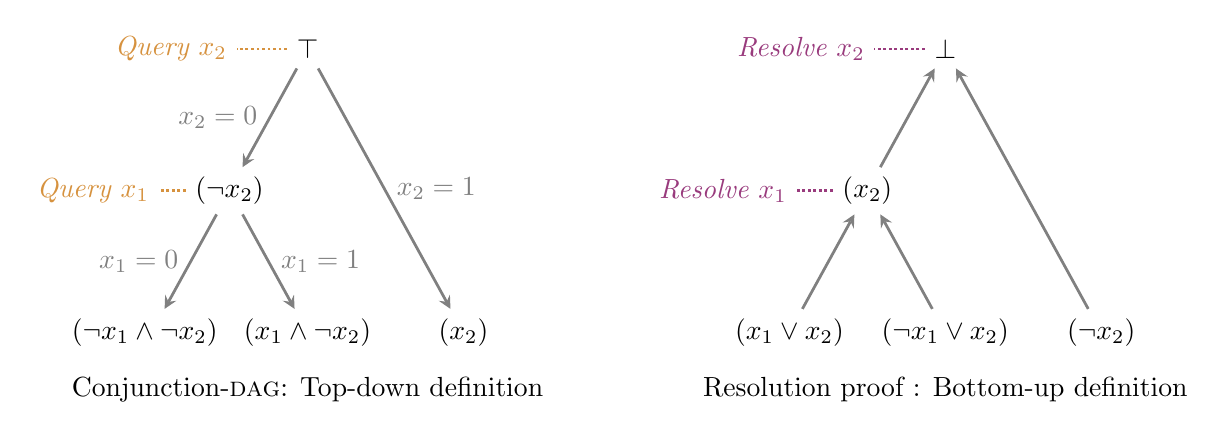
\begin{tikzpicture}[scale=0.9]
	\def \rootx {9}
	\def \rooty {0}
	\tikzstyle{resedge} = [-stealth,line width=1pt,pos=0.35,inner sep=4,color=gray]
	\newcommand{\resolve}[2]{
		\draw[densely dotted, line width=1pt, ColA] (#1) edge ([shift={(-1,0)}]#1);
		\node[left, ColA] at ([shift={(-1,0)}]#1) {{#2}};	
	}
	
	\node (root) at (\rootx,\rooty) {$\bot$};

	\node (a) at ([shift={(-1.1,-2)}]root) {$(x_2)$} edge[resedge] (root);	
	\node (b) at ([shift={(-1.1,-2)}]a) {$(x_1 \vee x_2)$} edge[resedge] (a);
	\node (c) at ([shift={(1.1,-2)}]a) {$(\lnot x_1 \vee x_2)$} edge[resedge] (a);
	\node (d) at ([shift={(2.2,-4)}]root) {$(\lnot x_2)$} edge[resedge] (root);
	\resolve{root}{\itshape Resolve $x_2$}
	\resolve{a}{\itshape Resolve $x_1$}
	\node at ([shift={(0,-4.8)}]root) {Resolution proof : Bottom-up definition};
	
	\def \rootx {0}
	\def \rooty {0}
	\tikzstyle{queryedge} = [stealth-,line width=1pt,pos=0.35,inner sep=4,color=gray]
	\newcommand{\query}[2]{
		\draw[densely dotted, line width=1pt, ColB] (#1) edge ([shift={(-1,0)}]#1);
		\node[left, ColB] at ([shift={(-1,0)}]#1) {{#2}};	
	}
	
	\node (root) at (\rootx,\rooty) {$\top$};
	\node (a) at ([shift={(-1.1,-2)}]root) {$(\lnot x_2)$} edge[queryedge] node [midway, left] {$x_2 = 0$} (root);
	\node (b) at ([shift={(-1.1,-2)}]a) {$(\lnot x_1 \wedge \lnot x_2)\enspace$} edge[queryedge] node [midway, left] {$x_1 = 0$} (a);
	\node (c) at ([shift={(1.1,-2)}]a) {$(x_1 \wedge \lnot x_2)$} edge[queryedge] node [midway, right] {$x_1 = 1$} (a);
	\node (d) at ([shift={(2.2,-4)}]root) {$(x_2)$} edge[queryedge] node [midway, right] {$x_2 = 1$} (root);
	\query{root}{\itshape Query $x_2$}
	\query{a}{\itshape Query $x_1$}
	\node at ([shift={(0,-4.8)}]root) {Conjunction-\DAGspace : Top-down definition};
\end{tikzpicture}
\end{center}
\vspace{-5mm}
\caption{Two equivalent ways to view a Resolution refutation, illustrated in the tree-like case (see \cite[\S18.2]{jukna12boolean} for more discussion of the tree-like case).}%
\label{fig:comparison}%
\end{figure}


\bigskip\noindent
The complexity measures introduced so far are related as follows; here $S'$ is \emph{any} two-party version of $S$ obtained by choosing some bipartition $\calX\times\calY=\{0,1\}^n$ of the 
input domain of $S$. %
\begin{equation} \label{eq:width-bound}
\rectDag(S')~\leq~\conjDag(S)~\leq~n^{O(w(S))}.
\end{equation}
The first inequality holds because each conjunction can be simulated by a rectangle. The second inequality holds since there are at most $n^{O(w)}$ many distinct width-$w$ conjunctions, and we may assume w.l.o.g.\ that any $f\in\calF$ is associated with at most one node in an $\calF$-\DAGspace (any incoming edge to a node $v$ can be rewired to the \emph{lowest} node $u$, in topological order, such that $f_v=f_u$).

\section{Our results} \label{sec:results}

Our first theorem is a characterization of the rectangle-\DAGspace complexity for \emph{composed} search problems of the form $S\circ g^n$. Here $S\subseteq\{0,1\}^n\times\calO$ is an arbitrary $n$-bit search problem, and~$g\colon\calX\times\calY\to\{0,1\}$ is some carefully chosen two-party \emph{gadget} that helps to distribute each input variable of $S$ between the two parties. More precisely, $S\circ g^n\subseteq \calX^n\times\calY^n\times\calO$ is the search problem where Alice holds $x\in\calX^n$, Bob holds $y\in\calY^n$, and their goal is to find some $o\in S(z)$ for $z\coloneqq g^n(x,y)=(g(x_1,y_1),\ldots,g(x_n,y_n))$.

Our concrete choice for a gadget is the usual $m$-bit \emph{index} function $\Ind_m\colon[m]\times\{0,1\}^m\to\{0,1\}$ mapping $(x,y)\mapsto y_x$. For large enough $m$, we show that the bounds \eqref{eq:width-bound} are tight.
\begin{theorem} \label{thm:main}
Let $m=m(n)\coloneqq n^\Delta$ for a large enough constant $\Delta$. For any $S\subseteq\{0,1\}^n\times \calO$,
\[
\rectDag(S\circ \Ind_m^n)~=~
n^{\Theta(w(S))}.
\]
\end{theorem}
We note that the conjunction-\DAGspace width complexity of $S\circ\Ind_m^n$ depends on how Alice's gadget inputs $x_i\in [m]$ are encoded as binary variables. For example, we can have $w(S\circ\Ind_m^n)=\Theta(w(S))$ when using a ``unary'' encoding; see \autoref{sec:apps} for a discussion. 


\paragraph{Implications.}
The primary advantage of such a lifting theorem is that we obtain, in a generic fashion, a large class of hard (explicit) monotone functions and CNF contradictions. Let us outline how to apply our theorem. We can start with any $n$-variable $k$-CNF contradiction $F$ of Resolution width~$w$, and conclude from \autoref{thm:main} that the composed problem $S'\coloneqq S_F\circ\Ind^n_m$ has rectangle-\DAGspace complexity $n^{\Theta(w)}$. Then we can use reductions (either new or known; see \autoref{sec:apps} for known ones) to translate $S'$ back to a mKW/CNF search problem. The upshot will be 
%
the following.   %
\begin{itemize}
\item $S'$ reduces to $S_{f'}$ where $f'$ is some $N$-bit monotone function with $N\coloneqq n^{O(k)}$.
\item $S'$ reduces to $S_{F'}$ where $F'$ is some $n^{O(1)}$-variable $2k$-CNF contradiction. 
\end{itemize}

A follow-up
%
article~\cite{goos19monotone}  %
has provided concrete applications using a novel reduction framework based on the above template. For example, they consider a monotone function $\ThreeXorSat_n\colon\bit^N\to\bit$ over $N\coloneqq 2n^3$ input bits defined as follows. An input $x\in\bit^N$ is interpreted as (the indicator vector of) a set of $\ThreeXor$ constraints over $n$ boolean variables $v_1,\ldots,v_n$ (there are $N$ possible constraints). We define $\ThreeXorSat_n(x)\coloneqq 1$ iff the set~$x$ is \emph{unsatisfiable}, that is, no boolean assignment to the~$v_i$ exists that satisfies all constraints in $x$. They proceed to show that if $F$ is an $n$-variable ``Tseitin'' contradiction (which is hard for Resolution~\cite{urquhart87hard}), then $S'=S_F \circ \Ind_m^n$ reduces to~$S_{\ThreeXorSat_{mn}}$. Combining this with \autoref{thm:main}, one obtains the following.

\begin{corollary}[{\cite[Thm.~1]{goos19monotone}}]\label{cor:xorsat-lb}
$\ThreeXorSat_n$ requires monotone circuits of size $2^{n^{\Omega(1)}}$.
\end{corollary}

Since $\ThreeXorSat_n$ is in $\NC^2$~\cite{mulmuley87fast}, this improves on the exponential monotone vs.\ non-mono\-tone separation due to Tardos~\cite{tardos88gap}; her function is in $\Pc$ and not known to be in $\NC$.


\paragraph{Limitations.}
A disadvantage, stemming from the large gadget size $m=n^\Delta$, is that we get at best (using $w=\Theta(n)$) a monotone circuit lower bound of~$\exp(N^{\varepsilon})$ for a small constant $\varepsilon\geq 1/(\Delta+1)$. Such lower bounds fall short of the current best record of $\exp(N^{1/3-o(1)})$ due to Harnik and Raz~\cite{harnik00higher}. We inherit the need for large gadgets from prior work \cite{goos16rectangles,goos17bpp}; see \autoref{sec:tools}. For this reason (and others), it is an important open problem to develop a lifting theory for gadgets of size $m=O(1)$. In particular, an optimal~$2^{\Omega(N)}$ lower bound would follow from an appropriate constant-size-gadget version of \autoref{thm:main}; see \autoref{sec:apps} for details.


\paragraph{Techniques.}
We use tools developed in the context of tree-like lifting theorems, specifically from~\cite{goos16rectangles,goos17bpp}. These tools allow us to relate large rectangles in the input domain of $S\circ\Ind_m^n$ with large subcubes in the input domain of $S$; see \autoref{sec:tools}. Given these tools, the proof of \autoref{thm:main} is relatively short (two pages). The proof is extremely direct: from any rectangle-\DAGspace of size $n^d$ solving $S\circ \Ind^n_m$ we extract a width-$O(d)$ conjunction-\DAGspace solving $S$.

Classical
%
work     %
on monotone circuit lower bounds
%
has      %
typically focused on specific monotone functions~\cite{razborov85monlower,andreev1985monlower,alon87monlower,haken95bottleneck,rossman14monotone} and more generally on studying the power of the underlying proof methods~\cite{razborov89onthemethod,wigderson93thefusion,razborov97generalapprox,simon97approxbottle,berg99approxbottle,amano04approxbottle}. A notable exception is Jukna's criterion~\cite{jukna97finitelimits}, recently applied in~\cite{hrubes17randomformulas,fleming17randomcnf}, which is a general sufficient condition for a monotone function to require large monotone circuit complexity. Our perspective is seemingly even more abstract, as our result is phrased for arbitrary search problems (not just of mKW/CNF type). However, it remains unclear exactly how the power of our methods compare with the classical techniques; for example, can our result be rephrased in the language of Razborov's method of approximations? (An anonymous reviewer thinks this is possible, but not instructive.)


\begin{figure}
\centering
%
\begin{lpic}[t(-8mm),l(-9mm),r(-9mm),b(-5mm)]{shapes(.41)}
\normalsize
\lbl[c]{60,7;(a)}
\lbl[c]{160,7;(b)}
\lbl[c]{260,7;(c)}
\lbl[c]{360,7;(d)}
\end{lpic}
\caption{We show lifting theorems for \DAGs whose feasible sets are (a) \emph{rectangles} or (b) \emph{triangles}. It remains open (see \autoref{sec:open}) to prove any lower bounds for explicit mKW/CNF search problems when the feasible sets are (c)~\emph{block-diagonal}, which a special case of (d) \emph{intersections of 2 triangles}.}
\label{fig:shapes}
\end{figure}


\subsection{Extension: Monotone real circuits}

\paragraph{Triangle-\DAGs.}
Consider a bipartite input domain $\calI\coloneqq \calX\times\calY$ and let $\calF$ be the set of all indicator functions of \emph{(combinatorial) triangles over~$\calX\times\calY$}; here a \emph{triangle} $T\subseteq\calX\times\calY$ is a set that can be written as $T= \{(x,y)\in\calX\times\calY: a_T(x)<b_T(y)\}$ for some labeling of the rows $a_T \colon \calX \to \mathbb{R}$ and columns~$b_T\colon\calY \to \mathbb{R}$ by real numbers; see \hyperref[fig:shapes]{\expref{Figure}{fig:shapes}b}. In particular, every rectangle is a triangle. Call such $\calF$-\DAGs simply \emph{triangle-\DAGs}. For a search problem $S\subseteq \calX\times\calY\times\calO$ we define
\[
\triDag(S)~\coloneqq~\text{least \emph{size} of a triangle-\DAGspace that solves $S$}.
\]

Hrube{\v{s}} and Pudl{\'a}k~\cite{hrubes17note} showed recently that the \emph{monotone real circuit complexity} of an~$f$ equals $\triDag(S_f)$. Monotone real circuits~\cite{haken99exponential,pudlak97lower} generalize monotone circuits by allowing the wires to carry arbitrary real numbers and the binary gates to compute arbitrary monotone functions $\mathbb{R}\times\mathbb{R}\to\mathbb{R}$. The original motivation to study such circuits, and what interests us here, is that lower bounds for monotone real circuits imply lower bounds for the \emph{Cutting Planes} proof system~\cite{cook87complexity}. In our language, semantic Cutting Planes refutations are equivalent to $\calL$-\DAGs solving CNF search problems, where $\calL$ is the family of linear threshold functions (each $f\in\calL$ is defined by some $(n+1)$-tuple $a\in\mathbb{R}^{n+1}$ so that $f(x)=1$ iff $\sum_{i\in[n]} a_ix_i > a_{n+1}$).

\bigskip\noindent
Our second theorem states that \autoref{thm:main} holds more generally with rectangle-\DAGs replaced with triangle-\DAGs. The proof is however more involved than the proof for \autoref{thm:main}.
\begin{theorem} \label{thm:triangle}
Let $m=m(n)\coloneqq n^\Delta$ for a large enough constant $\Delta$. For any $S\subseteq\{0,1\}^n\times \calO$,
\[
\triDag(S\circ \Ind_m^n)~=~
n^{\Theta(w(S))}.
\]
\end{theorem}

A pithy corollary is that if we start with any $k$-CNF contradiction $F$ that is hard for Resolution and compose $F$ with a gadget (as described in \autoref{sec:apps}), the formula becomes hard for Cutting Planes. In particular, the composed formula can itself be written as a $2k$-CNF.

\begin{corollary}\label{cor:cutting-lb}
For any unsatisfiable $k$-CNF $F$ on $n$ variables, there is a related unsatisfiable $2k$-CNF $F'$ on $n^{O(1)}$ variables, such that any Cutting Planes refutation for $F'$ has length at least $n^{\Omega(w(S_F))}$.
\end{corollary}

The follow-up %
article \cite{goos19monotone} %
observed a near-immediate corollary: the Nullstellensatz proof system (over any field) can be exponentially more powerful than Cutting Planes.

\begin{corollary}[{\cite[\S4.2]{goos19monotone}}]\label{cor:cp-vs-ns}
There exists an $n$-variable, $n^{O(1)}$-clause CNF contradiction $F$ that can be refuted by Nullstellensatz (over any field) in degree $O(\log n)$, but that requires Cutting Planes refutations of length $2^{n^{\Omega(1)}}$.
\end{corollary}

Previously, only few examples of hard contradictions were known for Cutting Planes, all proved via feasible interpolation~\cite{pudlak97lower,haken99exponential,hrubes17randomformulas,fleming17randomcnf}. A widely-asked question has been to improve this state-of-the-art by developing alternative lower bound methods; see the surveys~\cite[\S4]{beame01propositional} and~\cite[\S5]{razborov16proof}. In particular, Jukna~\cite[Research Problem 19.17]{jukna12boolean} asked to find a more intuitive ``combinatorial'' proof method ``explicitly showing what properties of [contradictions] force long derivations.'' While our method does implicitly use feasible interpolation for Cutting Planes, at least it does afford a simple combinatorial intuition: the hardness is simply borrowed from the realm of Resolution (where we understand very well what makes formulas hard).


\section{Subcubes from rectangles} \label{sec:tools}

In this section, as preparation, we recall some technical notions from~\cite{goos16rectangles,goos17bpp} concerning the index gadget $g\coloneqq \Ind_m$.
%
Specifically,  %
writing $G\coloneqq g^n\colon\allX\times\allY\to\{0,1\}^n$ for $n$ copies of $g$, we explain how large rectangles in
the domain of $G$ %
are related with large subcubes in
the codomain of $G$. %
In what follows, we will always assume that $m \ge n^\Delta$ for a sufficiently large constant $\Delta$.

\subsection{Structured rectangles}
For a partial assignment $\rho\in\{0,1,*\}^n$ we let $\free\rho\coloneqq \rho^{-1}(*)$ denote its \emph{free} coordinates, and $\fix\rho\coloneqq[n]\smallsetminus\free\rho$ denote its \emph{fixed} coordinates. The number of fixed coordinates $|\!\fix\rho|$ is the \emph{width} of $\rho$. Width-$d$ partial assignments are naturally in 1-to-1 correspondence with width-$d$ conjunctions: for any $\rho$ we define $C_\rho\colon \{0,1\}^n\to\{0,1\}$ as the width-$|\!\fix\rho|$ conjunction that accepts an $x\in\{0,1\}^n$ iff $x$ is consistent with~$\rho$. Thus $C_\rho^{-1}(1)=\{x\in\{0,1\}^n: x_i = \rho_i \text{ for all } i \in \fix\rho\}$ is a subcube. We say that $R\subseteq\allX\times\allY$ is \emph{$\rho$-like} if the image of $R$ under $G$ is precisely the subcube of $n$-bit strings consistent with $\rho$, that is,
\[
R \text{ is \emph{$\rho$-like}}
\quad\iff\quad G(R)~=~C_\rho^{-1}(1).
\]


For a random variable $\x$ we let $\Hmin(\x)\coloneqq\min_x \log(1/\Pr[\x=x])$ denote the usual \emph{min-entropy} of $\x$. When $\x\in[m]^J$ for some index set $J$, we write $\x_I\in[m]^I$ for the marginal distribution of $\x$ on a subset $I\subseteq J$ of coordinates. For a set $X$ we use the boldface $\X$ to denote a random variable uniformly distributed over~$X$.


\begin{definition}[\cite{goos16rectangles}]
A random variable $\x\in[m]^J$ is \emph{$\delta$-dense} if for every nonempty $I\subseteq J$, $\x_I$ has \emph{min-entropy rate} $\geq \delta$, that is, $\Hmin(\x_I) \geq \delta\cdot |I|\log m$.
\end{definition}
\begin{definition}[\cite{goos17pnp,goos17bpp}] \label{def:structured}
A rectangle $R\coloneqq X\times Y\subseteq\allX\times\allY$ is \emph{$\rho$-structured} if
\begin{enumerate}
\item $\X_{\fix \rho}$ is fixed, and every $z\in G(R)$ is consistent with $\rho$, that is, $G(R)\subseteq C_\rho^{-1}(1)$;
\item $\X_{\free \rho}$ is \emph{$0.9$-dense};
\item $Y$ is large enough: $\Hmin(\Y)\geq mn-n^3$.
\end{enumerate}
\end{definition}


\begin{lemma}[\cite{goos17pnp,goos17bpp}] \label{lem:gadget}
For $m \ge n^\Delta$, every $\rho$-structured rectangle is $\rho$-like.
\end{lemma}

In this %
article   %
we need a slight strengthening of \expref{Lemma}{lem:gadget}: for a $\rho$-structured $R$, there is a \emph{single row} of $R$ that is already $\rho$-like. The proof of the following lemma is defered to \autoref{sec:row-lem-proof}.

\begin{lemma} \label{lem:row}
Let $X\times Y$ be $\rho$-structured. For $m \ge n^\Delta$, there exists $x\in X$ such that $\{x\}\times Y$ is $\rho$-like.
\end{lemma}

We remark that the \emph{only} reason why our proofs require $m \ge n^\Delta$ is due to \expref{Lemma}{lem:row}.

\begin{figure}[t]
	\centering
%
	\begin{lpic}[t(-4mm),b(-2mm)]{scheme(.41)}        
		\large
		\lbl[c]{7,60;$X$}
		\lbl[c]{70,112;$Y$}
		\lbl[c]{165,27.5;$X_{\err}$}
		\lbl[c]{272.5,112;$Y_{\err}$}
		\normalsize
		\lbl[c]{70,7;(a)}
		\lbl[c]{230,7;(b)}
	\end{lpic}
	\caption{(a) \rectscheme partitions $R=X\times Y$ first along rows, then along columns. (b)~\rectlemma illustrated: most subrectangles are $\rho$-structured for low-width $\rho$, except some error parts (highlighted in figure) that are contained in few error rows/columns $X_{\err}$, $Y_{\err}$.}
	\label{fig:scheme}
\end{figure}

\subsection{Rectangle partition scheme}

We claim that, given any rectangle $R \coloneqq X\times Y\subseteq \allX\times\allY$, we can partition most of $X\times Y$ into $\rho$-structured subrectangles with $|\!\fix\rho|$ bounded in terms of the size of $X\times Y$. Indeed, we describe a simple 2-round partitioning scheme from~\cite{goos17bpp} below; see also \autoref{fig:scheme}. In the 1st round of the algorithm, we partition the rows as $X=\bigsqcup_i X^i$ where each $X^i$ will be fixed on some blocks $I_i\subseteq[n]$ and $0.95$-dense on the remaining blocks~$[n]\smallsetminus I_i$. In the 2nd round, each $X^i\times Y$ is further partitioned along columns so as to fix the outputs of the gadgets on coordinates $I_i$.

\vspace{1mm}

\floatname{algorithm}{Rectangle Scheme}
\begin{algorithm}[ht]
	\begin{algorithmic}[1]
		\vspace{1mm}
		\Input $R = X \times Y \subseteq \allX \times \allY$.
		\Output A partition of $R$ into subrectangles.
		\vspace{2mm}
		\State {\bf 1st round:}~ Iterate the following for $i=1,2,\ldots,$ until $X$ becomes empty:
	\begin{enumerate}[label=(\roman*),topsep=1mm]
		\item Let $I_i\subseteq [n]$ be a \emph{maximal} subset (possibly $I_i=\emptyset$) such that $\X_{I_i}$ has min-entropy rate $<0.95$, and let $\alpha_i\in[m]^{I_i}$ be an outcome witnessing this: $\Pr[\X_{I_i}=\alpha_i]>m^{-0.95|I_i|}$
		\item Define $X^i \coloneqq \set{x \in X: x_{I_i}=\alpha_i}$
		\item Update $X \gets X \smallsetminus X^i$
	\end{enumerate}
\vspace{1mm}
\State {\bf 2nd round:}~ For each part $X^i$ and $\gamma \in \bit^{I_i}$, define $Y^{i,\gamma} \coloneqq \{ y \in Y : g^{I_i}(\alpha_i,y_{I_i})=\gamma\}$
\vspace{1mm}
\State \Return $\set{R^{i,\gamma} \coloneqq X^i \times Y^{i,\gamma} : Y^{i,\gamma} \ne \emptyset}$
	\end{algorithmic}
	\caption{\vspace{.5mm}}
	\label{alg:partition}
\end{algorithm}

All the properties of \rectscheme that we will subsequently need are formalized below; see also \autoref{fig:scheme}. For terminology, given a subset $A'\subseteq A$ we define its \emph{density} (inside $A$) as $|A'|/|A|$. The proof of the following lemma is postponed to \autoref{sec:proof-rect-partition}.

\begin{lemma}[Rectangle Lemma] \label{lem:scheme}  %
\em Fix any parameter $k \leq n \log n$. Given a rectangle $R\subseteq \allX\times\allY$, let $R=\bigsqcup_i R^i$ be the output of \rectscheme. Then there exist ``error'' sets $X_{\err}\subseteq \allX$ and $Y_{\err}\subseteq\allY$, both of density $\leq 2^{-k}$, such that for each $i$, one of the following holds:
\begin{itemize}[label=$\bullet$,itemsep=1mm]
\item {\bf\slshape Structured case:}~ $R^i$ is $\rho^i$-structured for some $\rho^i$ of width at most $O(k/\log n)$.
\item {\bf\slshape Error case:}~ $R^i$ is covered by error rows/columns, \ie, $R^i\subseteq X_{\err}\times \allY\cup \allX\times Y_{\err}$.
\end{itemize}
Finally, a {\bf\itshape query alignment} property holds: for every $x \in \allX\smallsetminus X_{\err}$, there exists a subset $I_x \subseteq [n]$ with $|I_x| \le O(k/\log n)$ such that every ``structured'' $R^i$ intersecting $\set{x} \times \allY$ has $\fix \rho^i \subseteq I_x$.
\end{lemma}


\section{Lifting for rectangle-\DAGs} \label{sec:proof-rect}

In this section we prove the nontrivial direction of \autoref{thm:main}: Let $\Pi$ be a rectangle-\DAGspace solving $S\circ G$ of size $n^d$ for some~$d$. Our goal is to show that $w(S)\leq O(d)$.

\subsection{Game semantics for \DAGs}
For convenience (and fun), we use the language of two-player competitive games, introduced in~\cite{pudlak00proofs,atserias08combinatorial}, which provide an alternative way of thinking about conjunction-\DAGs solving $S\subseteq\{0,1\}^n\times \calO$. The game involves two competing players, \emph{Explorer} and \emph{Adversary}, and proceeds in rounds. The state of the game in each round is modeled as a partial assignment $\rho\in\{0,1,*\}^n$. At the start of the game, $\rho\coloneqq *^n$. In each round, Explorer makes one of two moves:
\begin{itemize}
\item \emph{Query a variable:}~ Explorer specifies an $i\in\free\rho$, and Adversary responds with a bit $b\in\{0,1\}$. The state $\rho$ is updated by $\rho_i \leftarrow b$.
\item \emph{Forget a variable:}~ Explorer specifies an $i\in\fix\rho$, and the state is updated by $\rho_i\leftarrow *$.
\end{itemize}
An important detail is that Adversary is allowed to choose $b\in\{0,1\}$ afresh even if the $i$-th variable was queried and subsequently forgotten during past play. The game ends when a solution to $S$ can be inferred from $\rho$, that is, when $C_\rho^{-1}(1)\subseteq S^{-1}(o)$ for some $o\in \calO$.

Explorer's goal is to end the game while keeping the width of the game state $\rho$ as small as possible. Indeed, Atserias and Dalmau~\cite{atserias08combinatorial} prove that $w(S)$ is characterized (up to an additive~$\pm 1$) as the least $w$ such that the Explorer has a strategy for ending the game that keeps the width of the game state at most $w$ throughout the game. (A similar characterization exists for \DAGspace \emph{size}~\cite{pudlak00proofs}.) Hence our goal becomes to describe an Explorer-strategy for $S$ such that the width of the game state never exceeds $O(d)$ regardless of how the Adversary plays.

\subsection{Simplified proof} \label{sec:simple-proof}

To explain the basic idea, we first give a simplified version of the proof: We assume that all rectangles~$R$ involved in~$\Pi$---call them the \emph{original} rectangles---can be partitioned \emph{errorlessly} into $\rho$-structured subrectangles for $\rho$ of width $O(d)$. That is, invoking \rectscheme for each original~$R$, we assume that
\begin{enumerate}[label=($\bm{*}$)]
\item \label{assumption}
\emph{Assumption:}~ All subrectangles in the partition $R=\bigsqcup_i R^i$ output by \rectscheme satisfy the ``structured'' case of \rectlemma for $k\coloneqq 2d\log n$.
\end{enumerate}
In \autoref{sec:error} we remove this assumption by explaining how the proof can be modified to work in the presence of some error rows/columns.

\paragraph{Overview.}
We extract a width-$O(d)$ Explorer-strategy for $S$ by walking down the rectangle-\DAG~$\Pi$, starting at the root. For each original rectangle $R$ that is reached in the walk, we maintain a $\rho$-structured subrectangle $R'\subseteq R$ chosen from the partition of $R$. Note that $\rho$ will have width $O(d)$ by our choice of $k$. The intention is that $\rho$ will record the current state of the game. There are three issues to address: (1) Why is the starting condition of the game met? (2) How do we take a step from a node of $\Pi$ to one of its children? (3) Why are we done once we reach a leaf?

\paragraph{(1) Root case.}
At start, the root of $\Pi$ is associated with the original rectangle $R=\allX\times\allY$ comprising the whole domain. The partition of $R$ computed by \rectscheme is trivial: it contains a single part, the $*^n$-structured $R$ itself. Hence we simply maintain the $*^n$-structured $R\subseteq R$, which meets the starting condition for the game.

\paragraph{(2) Internal step.}
This is the crux of the 
argument. %
Supposing the game has reached state $\rho_{R'}$ and we are maintaining some $\rho_{R'}$-structured subrectangle $R'\subseteq R$ where $R$ is associated with an internal node $v$, we want to move to some $\rho_{L'}$-structured subrectangle $L'\subseteq L$ where $L$ is associated with a child of $v$. We must keep the width of the game state at most $O(d)$ during this move.

\begin{center}
%
\begin{lpic}[t(-6mm),b(-8mm)]{internal-step(.35)}
\definecolor{myGold}{RGB}{231,141,20}
\definecolor{myBlue}{rgb}{0.19,0.41,.65}
\definecolor{myPurple}{RGB}{175,0,124}
\large
\lbl[c]{70,90;\color{myBlue}$R'$}
\lbl[c]{310,130;\color{myGold}$L_1$}
\lbl[c]{30,120;\color{myGold}$L_0$}
\normalsize
\lbl[c]{215,117;$Y'$}
\lbl[c]{277,70;$X'$}
\lbl[r]{56,62;\color{myPurple}$x^*$}
\lbl[c]{121,69;\color{myPurple}$(x^*,y^*)$}
\end{lpic}
\end{center}

Since $R' \eqqcolon X' \times Y'$ is $\rho_{R'}$-structured, we have from \expref{Lemma}{lem:row} that there exists some $x^*\in X'$ such that $\{x^*\}\times Y'$ is $\rho_{R'}$-like. Let the two original rectangles associated with the children of $v$ be $L_0$ and $L_1$. Let $\bigsqcup_i L_b^i$ be the partition of $L_b$ output by \rectscheme. By query alignment in \rectlemma, there is some $I_b^*\subseteq [n]$, $|I_b^*|\leq O(d)$, such that all $L_b^i$ that intersect the $x^*$-th row are $\rho^i$-structured with $\fix\rho^i\subseteq I_b^*$. As Explorer, we now query the input variables in coordinates $J\coloneqq (I_0^* \cup I_1^*) \smallsetminus \fix\rho_{R'}$ (in any order) obtaining some response string $z_J\in\{0,1\}^J$ from the Adversary. As a result, the state of the game becomes the extension of $\rho_{R'}$ by $z_J$, call it $\rho^*$, which has width $|\!\fix\rho^*|=|\!\fix\rho_{R'}\cup J|\leq O(d)$.

Note that there is some $y^*\in Y'$ (and hence $(x^*, y^*) \in R'\subseteq L_0\cup L_1$) such that $G(x^*,y^*)$ is consistent with~$\rho^*$; indeed, the whole row $\{x^*\}\times Y'$ is $\rho_{R'}$-like and $\rho^*$ extends $\rho_{R'}$. Suppose $(x^*, y^*) \in L_0$; the case of $L_1$ is analogous. In the partition of $L_0$, let $L'$ be the unique part such that $(x^*,y^*)\in L'$. Note that $L'$ is $\rho_{L'}$-like for some $\rho_{L'}$ that is consistent with $G(x^*,y^*)$ and $\fix\rho_{L'}\subseteq I_0^*$ (by query alignment). Hence $\rho^*$ extends $\rho_{L'}$. As Explorer, we now forget all queried variables in $\rho^*$ except those queried in $\rho_{L'}$.

We have recovered our invariant: the game state is $\rho_{L'}$ and we maintain a $\rho_{L'}$-structured subrectangle $L'$ of an original rectangle $L_0$. Moreover, the width of the game state remained $O(d)$.

\paragraph{(3) Leaf case.}
Suppose the game state is $\rho$ and we are maintaining an associated $\rho$-structured subrectangle $R'\subseteq R$ corresponding to a \emph{leaf} node. The leaf node is labeled with some solution $o\in \calO$ satisfying $R'\subseteq (S\circ G)^{-1}(o)$, that is, $G(R')\subseteq S^{-1}(o)$. But $G(R')=C_\rho^{-1}(1)$ by \expref{Lemma}{lem:gadget} so that $C_\rho^{-1}(1)\subseteq S^{-1}(o)$. Therefore the game ends. This concludes the (simplified) proof.


\subsection{Accounting for error} \label{sec:error}

Next, we explain how to get rid of
%
Assumption~\ref{assumption}  %
by accounting for the rows and columns that are classified as error in \rectlemma for $k\coloneqq 2d\log n$. The partitioning of
rectangles in $\Pi$ %
is done more
carefully.  %
We sort all original rectangles in \emph{reverse topological order} $R_1,R_2,\ldots,R_{n^d}$ from leaves to root, that is, if $R_i$ is a descendant of $R_j$ then $R_i$ comes before $R_j$ in the order. Then we
perform the following %
process
on %
the rectangles
in this order. %

\medskip\noindent
{\slshape Initialize cumulative error sets $X^*_{\err}=Y^*_{\err}\coloneqq\emptyset$. Iterate for $i=1,2,\ldots,n^d$} rounds:
\begin{enumerate}[topsep=1mm,itemsep=2mm]
\item Remove from $R_i$ the rows/columns $X^*_{\err}$, $Y^*_{\err}$. That is, update
\[
R_i~\leftarrow~
R_i \smallsetminus \big(X^*_{\err}\times \allY \cup \allX\times Y^*_{\err}\big).
\]
\item Apply the \rectscheme for $R_i$. Output all resulting subrectangles that satisfy the ``structured'' case of \rectlemma for $k\coloneqq 2d\log n$. (All non-structured subrectangles are omitted). Call the resulting error rows/columns $X_{\err}$ and $Y_{\err}$.
\item Update $X^*_{\err}\leftarrow X^*_{\err} \cup X_{\err}$ and $Y^*_{\err}\leftarrow Y^*_{\err}\cup Y_{\err}$.
\end{enumerate}

\medskip\noindent
In words, an original rectangle $R_i$ is processed only after all of its descendants are partitioned. Each descendant may contribute some error rows/columns, accumulated into sets $X^*_{\err}$, $Y^*_{\err}$, which are deleted from $R_i$ before it is partitioned. The partitioning of $R_i$ will in turn contribute its error rows/columns to its ancestors.

We may now repeat the proof of \autoref{sec:simple-proof} verbatim \emph{using only the structured subrectangles output by the above process}. That is, we still maintain the same invariant: when the game state is $\rho$, we maintain a $\rho$-structured $R'$ (output by the above process) of an original $R$. We highlight only the key points below.

\paragraph{(1) Root case.}
The cumulative error at the end of the process is tiny: $X^*_{\err}$, $Y^*_{\err}$ have density at most $n^d\cdot n^{-2d}\leq 1\%$ by a union bound over all rounds. In particular, the root rectangle $R_{n^d}$ (with errors removed) still has density $98\%$ inside $\allX\times\allY$, and so the partition output by \rectscheme is trivial, containing only the $*^n$-structured $R_{n^d}$ itself. This meets the starting condition for the game.

\paragraph{(2) Internal step.}
By construction, the cumulative error sets \emph{shrink} when we take a step from a node to one of its children. This means that our error handling does not interfere with the internal step: each structured subrectangle $R'$ of an original rectangle $R$ is wholly covered by the structured subrectangles of
the children of $R$. %

\paragraph{(3) Leaf case.} This case is unchanged.


\section{Lifting for triangle-\DAGs} \label{sec:proof-tri}

In this section we prove the nontrivial direction of \autoref{thm:triangle}. %
Let $\Pi$ be a triangle-\DAGspace solving $S\circ G$ of size $n^d$ for some~$d$. Our goal is to show that $w(S)\leq O(d)$.

The proof is conceptually the same as for rectangle-\DAGs. The only difference is that we need to replace \rectscheme (and the associated \rectlemma) with an algorithm that partitions a given triangle $T\subseteq\allX\times\allY$ into subtriangles that behave like conjunctions.

\begin{figure}%
\begin{center}
%
\begin{lpic}[t(-6mm),b(-12mm)]{final-triangle(.35)}
\definecolor{myGold}{RGB}{231,141,20}
\definecolor{myBlue}{rgb}{0.19,0.41,.65}
\definecolor{myPurple}{RGB}{175,0,124}
\Large
\lbl[c]{38,105;\color{myPurple}$L^i$}
\lbl[c]{120,105;\color{myBlue}$T\cap R^i$}
\lbl[c]{225,34;\color{myGold}$R^i$}
\end{lpic}
\end{center}
\caption{Structured case of \trilemma: The subtriangle $T\cap R^i$ is sandwiched between two $\rho^i$-structured rectangles $L^i$ and $R^i$.}%
\label{fig:sandwich}%
\end{figure}


\subsection{Triangle partition scheme} \label{sec:trischeme-intro}

We introduce a triangle partitioning algorithm, \trischeme. Its precise definition is postponed to \autoref{sec:proof-tri-partition}. For now, we only need its high-level 
description. %
On input a triangle $T$, \trischeme outputs a disjoint cover $\bigsqcup_i R^i\supseteq T$ where $R^i$ are rectangles. This induces a partition of $T$ into subtriangles $T\cap R^i$. Each (non-error) rectangle $R^i$ is $\rho^i$-structured (for low-width $\rho^i$) and is associated with a $\rho^i$-structured ``inner'' subrectangle $L^i\subseteq R^i$ satisfying $L^i\subseteq T\cap R^i\subseteq R^i$; see \autoref{fig:sandwich}. Hence $T\cap R^i$ is $\rho^i$-like, as it is sandwiched between two $\rho^i$-like rectangles.

More formally, all the properties of \trischeme that we will subsequently need are formalized below (note the similarity with \rectlemma); see \autoref{sec:proof-trilemma} for the proof.

\begin{lemma}[Triangle Lemma]\label{lem:tri-scheme} %
  Fix any parameter $k \le n \log n$. Given a triangle $T\subseteq \allX\times\allY$, let $\bigsqcup_i R^i \supseteq T$ be the output of \trischeme. Then there exist ``error'' sets $X_{\err}\subseteq \allX$ and $Y_{\err}\subseteq\allY$, both of density $\leq 2^{-k}$, such that for each $i$, one of the following
holds. %
\begin{itemize}[label=$\bullet$,itemsep=1mm]
	\item {\bf\slshape Structured case:}~ $R^i$ is $\rho^i$-structured for some $\rho^i$ of width at most $O(k/\log n)$. Moreover, there exists an ``inner'' rectangle $L^i \subseteq T \cap R^i$ such that $L^i$ is also $\rho^i$-structured. 
	\item {\bf\slshape Error case:}~ $R^i$ is covered by error rows/columns, \ie, $R^i\subseteq X_{\err}\times \allY\cup \allX\times Y_{\err}$.
\end{itemize}
Finally, a {\bf\itshape query alignment} property holds: for every $x \in \allX\smallsetminus X_{\err}$, there exists a subset $I_x \subseteq [n]$ with $|I_x| \le O(k/\log n)$ such that every ``structured'' $R^i$ intersecting $\set{x} \times \allY$ has $\fix \rho^i \subseteq I_x$.
\end{lemma}


\subsection{Simplified proof}\label{sec:tri-simple-proof}

As in the rectangle case, we give a simplified proof assuming no errors. That is, invoking \trischeme for each triangle $T$ involved in $\Pi$, we assume that
\begin{enumerate}[label=($\bm{\dagger}$)]
\item \label{tri-assumption}
\emph{Assumption:} All rectangles in the cover $\bigsqcup_i R^i\supseteq T$ output by \trischeme satisfy the ``structured'' case of \trilemma for $k\coloneqq 2d\log n$.
\end{enumerate}

\noindent The argument for getting rid of the assumption \ref{tri-assumption} is the same as in the rectangle case, and hence we omit that step---one only needs to observe that removing cumulative error rows/columns from a triangle still leaves us with a triangle.

\paragraph{Overview.}
As before, we extract a width-$O(d)$ Explorer-strategy for $S$ by walking down the triangle-\DAG~$\Pi$, starting at the root. For each triangle $T$ of $\Pi$ that is reached in the walk, we maintain a $\rho$-structured inner rectangle $L\subseteq T$. Here $\rho$ (of width $O(d)$ by the choice of $k$) will record the current state of the game. There are the three steps (1)--(3) to address, of which (1) and (3) remain exactly the same as in the rectangle case. So we only explain step (2), which requires us to replace the use of \rectlemma with the new \trilemma.

\paragraph{(2) Internal step.}
Supposing the game has reached state $\rho_{L}$ and we are maintaining some $\rho_{L}$-structured inner rectangle $L\subseteq T$ associated with an internal node $v$, we want to move to some $\rho_{\widetilde{L}}$-structured inner rectangle $\widetilde{L}\subseteq \widetilde{T}$ associated with a child of $v$. Moreover, we must keep the width of the game state at most $O(d)$ during this move.
 

Since $L \eqqcolon X' \times Y'$ is $\rho_L$-structured, we have from \expref{Lemma}{lem:row} that there exists some $x^* \in X'$ such that $\{ x^*\} \times Y'$ is $\rho_L$-like. Let the two triangles associated with the children of $v$ be $T_0$ and $T_1$, so that $L\subseteq T_0\cup T_1$.

Let $\bigsqcup_i R_b^i$ be the rectangle cover of $T_b$ output by \trischeme. By query alignment in \trilemma, there is some $I_b^*\subseteq [n]$, $|I_b^*|\leq O(d)$, such that all $R_b^i$ that intersect the $x^*$-th row are $\rho^i$-structured with $\fix\rho^i\subseteq I_b^*$. As Explorer, we now query the input variables in coordinates $J \coloneqq (I_0^* \cup I_1^*) \smallsetminus \fix\rho_{L}$ (in any order) obtaining some response string $z_J\in\{0,1\}^J$ from the Adversary. As a result, the state of the game becomes the extension of $\rho_{L}$ by $z_J$, call it $\rho^*$, which has width $|\!\fix\rho^*|=|\!\fix\rho_{L}\cup J|\leq O(d)$.

Note that there is some $y^*\in Y'$ (and hence $(x^*,y^*)\in L\subseteq T_0\cup T_1$) such that $G(x^*,y^*)$ is consistent with~$\rho^*$; indeed, the whole row $\{x^*\}\times Y'$ is $\rho_{L}$-like and $\rho^*$ extends $\rho_{L}$. Suppose $(x^*, y^*) \in T_0$; the case of $T_1$ is analogous. In the rectangle covering of $T_0$, let $R$ be the unique part such that $(x^*,y^*)\in R$. Note that $R$ is $\rho_{R}$-like for some $\rho_{R}$ that is consistent with $G(x^*,y^*)$ and $\fix\rho_{R}\subseteq I_0^*$ (by query alignment). Hence $\rho^*$ extends $\rho_{R}$. As Explorer, we now forget all queried variables in $\rho^*$ except those queried in $\rho_{R}$. Also we move to the inner rectangle $\widetilde{L} \subseteq R$ promised by \trilemma that satisfies $\widetilde{L} \subseteq T_0$ and is $\rho_{\widetilde{L}} = \rho_R$ structured.

We have recovered our invariant: the game state is $\rho_{\widetilde{L}}$ and we maintain a $\rho_{\widetilde{L}}$-structured subrectangle $\widetilde{L}$ of a triangle $T_0$. Moreover, the width of the game state remained $O(d)$.


\section{Partitioning rectangles and triangles} \label{sec:proof-rect-partition}

In this section, we prove \rectlemma, define \trischeme, and prove \trilemma. We use repeatedly the following simple fact about min-entropy.
\begin{fact} \label{fact:basic}
Let $\X$ be a random variable and $E$ an event. Then $\Hmin(\X\mid E)\geq \Hmin(\X)-\log 1/\Pr[E]$.
\end{fact}

\subsection{Proof of Rectangle Lemma}

The proof is more-or-less implicit in \cite{goos16rectangles,goos17bpp}. We start by recording a key property of the 1st round of \rectscheme.

\begin{claim}\label{clm:density-restoring}
Each part $X^i$ obtained in 1st round of \rectscheme
%
satisfies the following conditions.  %
\begin{itemize}
\item \emph{Blockwise-density:}~ $\X^i_{[n] \smallsetminus I_i}$ is $0.95$-dense.
\item \emph{Relative size:}~ $|X^{\geqslant i}| \le m^{n - 0.05 |I_i|}$~ where $X^{\geqslant i} ~\coloneqq~ \bigcup_{j \ge i} X^j$.
\end{itemize}
\end{claim}
\begin{proof}
By definition, $\X^i = (\X^{\geqslant i}\, |\, \X^{\geqslant i}_{I_i} = \alpha_i)$. Suppose for contradiction that $\X^i_{[n] \smallsetminus I_i}$ is not $0.95$-dense. Then there is some nonempty subset $K \subseteq [n] \smallsetminus I_i$ and an outcome $\beta \in [m]^K$ violating the min-entropy condition, namely $\Pr[\X^i_K = \beta] > m^{-0.95 |K|}$. But this contradicts the maximality of $I_i$ since the larger set $I_i \cup K$ now violates the min-entropy condition for $\X^{\geqslant i}$:
\[
\Pr[\X^{\geqslant i}_{I_i \cup K} = \alpha_i \beta] ~=~ \Pr[\X^{\geqslant i}_{I_i} = \alpha_i] \cdot \Pr[\X^{i}_K = \beta] ~>~ m^{-0.95 |I_i|} \cdot m^{-0.95 |K|} ~=~ m^{-0.95(|I_i \cup K|)}\;.
\]
This shows the first property. For the second property, apply \autoref{fact:basic} for $\X^i = (\X^{\geqslant i}\, |\, \X^{\geqslant i}_{I_i} = \alpha_i)$ to find that $\Hmin(\X^i) \geq \Hmin(\X^{\geqslant i}) - 0.95|I_i|\log m$. On the other hand, since $\X^i$ is fixed on $I_i$, we have $\Hmin(\X^i)\leq (n-|I_i|)\log m$. Combining these two inequalities we get $\Hmin(\X^{\geqslant i}) \leq (n-0.05|I_i|)\log m$, which yields the second property.
\end{proof}

\paragraph{Proof of \rectlemma.}
\emph{Identifying $Y_{\err}$, $X_{\err}$.}
We define $Y_{\err} \coloneqq \bigcup_{i,\gamma} Y^{i,\gamma}$ subject to $|Y^{i,\gamma}| < 2^{mn-n^2}$. To bound the size of $Y_{\err}$, we claim that there are at most $(4m)^n$ possible choices of $i, \gamma$. Indeed, each $X^i$ is associated with a unique pair $(I_i \subseteq [n], \alpha_i \in [m]^{I_i})$, and there are at most $2^n$ choices of $I_i$ and at most $m^n$ choices of corresponding $\alpha_i$. Also, for each $X^i$, there are at most $2^n$ possible assignments to $\gamma \in \bit^{I_i}$. For each $i, \gamma$, we add at most $2^{mn - n^2}$ columns to $Y_{\err}$. Thus, $Y_{\err}$ has density at most $(4m)^n \cdot 2^{- n^2} < 2^{-k}$ inside $\allY$.
	
We define $X_{\err} \coloneqq \bigsqcup_i X^i$ subject to $|I_i| > 20 k/\log m$. Let $i$ be the least index with $|I_{i}| > 20k/\log m$ so that $X_{\err} \subseteq X^{\geqslant i}$. By \expref{Claim}{clm:density-restoring}, $|X^{\geqslant i}| \le m^{n - 0.05 |I_i|} < m^{n} \cdot 2^{-k}$ since $|I_i| > 20 k /\log m$. In other words, $X^{\geqslant i}$, and hence $X_{\err}$, has density at most $2^{-k}$ inside $\allX$.
	
\medskip\noindent
\emph{Structured vs.\ error.}
Let $R^{i,\gamma}\coloneqq X^i\times Y^{i,\gamma}$, where $X_i$ is associated with $(I_i,\alpha_i)$, be a rectangle \emph{not} contained in the error rows/columns. By definition of $X_{\err}$, $Y_{\err}$, this means $|Y^{i,\gamma}| \ge 2^{mn-n^2}$ (so that $\Hmin(\Y^{i,\gamma})\geq mn-n^2$) and $|I_i| \le 20 k/\log m$. We have from \expref{Claim}{clm:density-restoring} that $\X^i_{[n] \smallsetminus {I_i}}$ is $0.95$-dense. Hence, $R^{i,\gamma}$ is $\rho^i$-structured where $\rho^i$ equals $\gamma$ on $I_i$ and consists of stars otherwise.

\medskip\noindent
\emph{Query alignment.}
For each $x \in \allX \smallsetminus X_{\err}$, we define $I_x = I_i$ where $X^i$ is the unique part that contains $x$. It follows that any $\rho$-structured rectangle that intersects the $x$-th row is of the form $X^i \times Y^{i,\gamma}$ and hence has $\fix \rho = I_i$. Since $X^i \not\subseteq X_{\err}$, we have $|I_i| \le O(k/\log n)$.


\floatname{algorithm}{Triangle Scheme}
\begin{algorithm}[t]
	\begin{algorithmic}[1]
		\vspace{1mm}
		\Input Triangle $T \subseteq \allX \times \allY$ with labeling functions $(a_T, b_T)$
		\Output A disjoint rectangle cover $\bigsqcup_i R^i\supseteq T$
		\vspace{4mm}
		\State $Y_{\err} \gets \text{\columnclean on } T$
		\State Initialize~ $\calR^0_{\alive} \coloneqq \set{\allX \times (\allY \smallsetminus Y_{\err})}$;~~ $\calR^r_{\alive} \coloneqq \emptyset$ for all $r\geq 1$;~~ $\calR_{\final} \coloneqq  \emptyset$
		\vspace{2mm}
		\Loop ~for $r=0,1,2,\ldots,$ rounds until $\calR^r_{\alive}$ is empty:
		\ForAll {$R \in \calR^r_{\alive}$}
		\State $\bigsqcup_i R^i \gets$ \rectscheme on $R$ \underline{relative to free coordinates}
		\ForAll {parts $R^i$}
			\If {$|X^{T \cap R^i}| \ge |X^{R^i}|/2$}
			\State Add $R^i$ to $\calR_{\final}$
		\Else 
		\State
			$R^{i,\topp} \coloneqq $ top half of $R^i$ according to $a_T$~~(in particular $T\cap R^i\subseteq R^{i,\topp}$)
		\State Add $R^{i,\topp}$ to $\calR^{r+1}_{\alive}$ subject to $T \cap R^{i,\topp} \ne \emptyset$
		\EndIf
		\EndFor
		\EndFor
		\EndLoop
		\vspace{1.5mm}
		\State \Return $\calR_{\final} \cup \set{\allX \times Y_{\err}}$
	\end{algorithmic}
	\caption{}
	\label{alg:tri-partition}
\end{algorithm}


\subsection{Definition of Triangle Scheme} \label{sec:proof-tri-partition}

In the description of \trischeme, we denote projections of a set $S \subseteq \allX \times \allY$ by
\begin{align*}
X^S~&\coloneqq~\set{x \in \allX : \exists y \in \allY \text{ such that } (x,y) \in S},\\
Y^S~&\coloneqq~\set{y \in \allY : \exists x \in \allX \text{ such that } (x,y) \in S}.
\end{align*}
\paragraph{Overview.}
\trischeme computes a disjoint rectangle cover $\bigsqcup_i R^i$ of $T$. 
Starting with a trivial cover of the whole communication domain by a single part, the algorithm progressively \emph{refines} this cover over several rounds as guided by the input triangle $T$. As outlined in \autoref{sec:trischeme-intro}, the goal is to end up with $\rho$-structured rectangles $R^i$ that contain a large enough portion of $T$ so that we may sandwich $L^i\subseteq T\cap R^i\subseteq R^i$ where $L^i$ is a $\rho$-structured ``inner'' rectangle.

The main idea is as follows. The algorithm maintains a pool of \emph{alive} rectangles. In a single round, for each alive rectangle $R$, we first invoke \rectscheme in order to restore $\rho$-structuredness for the resulting subrectangles $R^i$. Then for each $R^i$ we check if the subtriangle $T\cap R^i$ occupies at least half the rows of~$R^i$. If \emph{yes}, we add it to the \emph{final} pool, which will eventually form the output of the algorithm. If \emph{no}, we discard the ``lower'' half of $R^i$ as determined by the labeling $a_T$, that is, the half that does not intersect $T$. The ``top'' half (containing $T\cap R^i$) will enter the alive pool for next round.

\paragraph{Column Cleanup.}
An important detail is the subroutine \columnclean, run at the start of \trischeme, which computes a small set of columns that will eventually be declared as $Y_{\err}$. By discarding the columns~$Y_{\err}$, we ensure that whatever subrectangle $R^i$ is
returned %
by \rectscheme, the rows of $T\cap R^i$ will satisfy an \emph{empty-or-heavy dichotomy}: for every $x\in X^{R^i}$, the $x$-th row of $T\cap R^i$ is either empty, or ``heavy'', that is, of size at least $2^{mn-n^2}$. For intuition, an extreme bad example we want to avoid is a triangle $T$ that is just a single column; such $T$ would be completely declared as ``error'' by \columnclean. Having many heavy rows helps towards satisfying the 3rd item in \autoref{def:structured} of $\rho$-stucturedness, and hence in finding the inner rectangle~$L^i$. This property of \columnclean is formalized in \expref{Claim}{clm:col-clean} below.

\paragraph{Free coordinates.}
Another detail to explain is the underlined phrase \emph{relative to free coordinates}. For each alive rectangle $R$ we tacitly associate a subset of \emph{free coordinates} $J_R\subseteq[n]$ and \emph{fixed coordinates} $[n]\smallsetminus J_R$. At start, the single alive rectangle has $J_R\coloneqq [n]$, and whenever we invoke \rectscheme for a rectangle $R$ \emph{relative to free coordinates}, the understanding is that in line (i) of \rectscheme, the choice of~$I_i$ is made among subsets of $J_R$ alone. The resulting subrectangle $R^i= X^i\times Y^i$, obtained by fixing the coordinates $I_i$ in~$X^i$, will have its free coordinates $J_{R^i}\coloneqq J_R\smallsetminus I_i$. (Restricting a rectangle to its top half on line 10 does not modify the free coordinates.)

\floatname{algorithm}{Column Clean-up}
\begin{algorithm}[t]
	\begin{algorithmic}[1]
		\vspace{1mm}
		\Input Triangle $T \subseteq \allX \times \allY$ with labeling functions $(a_T, b_T)$
		\Output Error columns $Y_{\err} \subseteq \allY$
		\vspace{4mm}
		\State $Y_{\err} \gets \emptyset$
		\State For $I \subseteq [n]$, $\alpha \in [m]^I$, $\gamma \in \bit^I$, define $Y_{I,\alpha,\gamma} \coloneqq \set{y \in \allY : g^I(\alpha, y_I) = \gamma}$
		\While {there exists $I, \alpha, \gamma, x$ such that $0 < |T \cap (\set{x} \times (Y_{I,\alpha,\gamma}\smallsetminus Y_{\err}))| < 2^{mn-n^2}$}
		\State $Y_{\err} \gets Y_{\err} \cup Y^{T \cap (\set{x} \times Y_{I,\alpha,\gamma})}$
		\EndWhile
		\State \Return $Y_{\err}$
	\end{algorithmic}
	\caption{}
	\label{alg:column-cleanup}
\end{algorithm}

\subsection{Properties of Triangle Scheme}

\begin{claim}\label{clm:col-clean}
For a triangle $T \subseteq \allX \times \allY$, let $Y_{\err}$ be the output of \columnclean. 
%
%
%
%
Then $Y_{\err}$ has the following properties. %
\begin{itemize}
	\item \emph{Empty-or-heavy:}~ For every triple $(I \subseteq [n], \alpha \in [m]^I, \gamma \in \bit^I)$, and every $x \in \allX$, it holds that $T \cap (\set{x} \times (Y_{I,\alpha,\gamma}\smallsetminus Y_{\err}))$ is either empty or has size at least $2^{mn-n^2}$.
	\item \emph{Size bound:}~ $|Y_{\err}| \le 2^{mn - \Omega(n^2)}$.
\end{itemize}
\end{claim}
\begin{proof}
The first property is immediate by definition of \columnclean. For the second property, in each while-iteration, at most $2^{mn-n^2}$ columns get added to $Y_{\err}$. Moreover, there are no more than $2^n \cdot m^n \cdot 2^n \cdot m^n = (2m)^{2n}$ choices of $I\subseteq [n]$, $\alpha \in [m]^I$, $\gamma \in \bit^I$ and $x \in [m]^n$, and the loop executes at most once for each choice of $I, \alpha, \gamma, x$. Thus, $|Y_{\err}| \le (2m)^{2n} \cdot 2^{mn - n^2} \le 2^{mn - \Omega(n^2)}$.
\end{proof}

Next, we list some key invariants that hold for \trischeme. 

\begin{lemma} \label{lem:invariants}
For every $r\geq 0$, there exists a partition $\calX^r \coloneqq \set{X^i}_i$ of $\allX$ satisfying the following.%
\begin{enumerate}[label={\upshape(P\arabic*)},leftmargin=13mm]
		\item \label{p1} For every $R \in \calR^r_{\alive}$ we have $X^R \in \calX^r$.
		\item \label{p2} Each $X^i \in \calX^r$ is labeled by a pair $(I_i \subseteq [n], \alpha_i \in [m]^{I_i})$ such that $\X^i_{I_i} = \alpha_i$ is fixed.
		\item \label{p3} The partition $\calX^{r+1}$ is a refinement of $\calX^r$. The labels respect this: if $X^j \in \calX^{r+1}$ is a subset of $X^i \in \calX^r$, then $I_j \supseteq I_i$ and $\alpha_j$ agrees with $\alpha_i$ on coordinates $I_i$.
\end{enumerate}
Moreover, let $\calX \coloneqq \calX^{r^*}$ be the final partition assuming \trischeme completes in $r^*$ rounds.
\begin{enumerate}[label={\upshape(P\arabic*)},leftmargin=13mm,resume]
		\item \label{p4} For every $R\in\calR_{\final}$ the row set $X^R$ is a union of parts of $\calX$. If $X^i\in\calX$, labeled $(I_i,\alpha_i)$, is such that $X^R\supseteq X^i$, then the fixed coordinates of $R$ are a subset of $I_i$.
		\item \label{p5}
		For every $r\geq0$, $\calX^r$ and $\calX$ agree on a fraction $\geq 1-2^{-r}$ of rows, that is, there is a subset of ``final'' parts $\calX^r_{\final}\subseteq\calX^r$ such that $\bigcup\calX^r_{\final}$ has density $\geq 1-2^{-r}$ inside $[m]^n$, and $\calX^r_{\final}\subseteq\calX$.
\end{enumerate}
\end{lemma}

\begin{proof}
Let us define the row partitions $\calX^r$.
The partition $\calX^1$ contains only a single part, $\allX$, labeled by $I_1\coloneqq \emptyset$. Supposing $\calX^r$ has been defined, the next partition $\calX^{r+1}$ is obtained by refining each old part $X^i\in\calX^r$. Consider one such old part $X^i\in\calX^r$ with label $(I_i,\alpha_i)$. If there is \emph{no} rectangle $R\in\calR^r_{\alive}$ with $X^R=X^i$ then we need not partition $X^i$ any further; we simply include $X^i$ in $\calX^{r+1}$ as a whole. Otherwise, let $R\in\calR^r_{\alive}$ be any rectangle such that $X^R=X^i$; we emphasize that there can be many such choices for $R$, but the upcoming refinement of $X^i$ will not depend on that choice. The $r$-th round of the algorithm first computes $R=\bigsqcup_i R^i$ using \rectscheme, and then each $R^i$ might be horizontally split in half. We interpret this as a refinement of $X^i$ according to the 1st round of \rectscheme on $R$ (which only depends on $X^R=X^i$), with each part adding more fixed coordinates to the label $(I_i, \alpha_i)$. Letting $X^i=\bigsqcup_j X^{i,j}$ denote the resulting row partition, we then split each $X^{i,j}$ into two halves $X^{i,j,\topp}$ and $X^{i,j,\bott}$. This completes the definition of $\calX^{r+1}$.

The properties \ref{p1}--\ref{p5} are straightforward to verify. For \ref{p5}, we only note that when the algorithm horizontally splits a rectangle (inducing $X^{i,j}=X^{i,j,\topp}\cup X^{i,j,\bott}$), the bottom halves are discarded, and never again touched in future rounds. That is, $X^{i,j,\bott}\in\calX^{r'}$ for all $r'>r$. This cuts the number of ``alive'' rows $\bigcup_{R\in\calR^r_{\alive}}\!\!X^R$ in half each round.
\end{proof}


\begin{lemma}[Error rows] \label{lem:tri-row-error-bound}
Let $\calX =\{X^i\}_i$ be the final row partition in \expref{Lemma}{lem:invariants}. Fix any parameter $k<n\log n$. There is a density-$2^{-k}$ subset $X_{\err} \subseteq [m]^n$ (which is a union of parts of $\calX$) such that for any part $X^i\not\subseteq X_{\err}$, we have $|I_i|\leq O(k/\log n)$.
\end{lemma}
\begin{proof}
Our strategy is as follows (cf.~\cite[Lemma 7]{goos17bpp}). For $x\in[m]^n$, let $i(x)$ be the unique index such that $x\in X^{i(x)}\in\calX$; recall that $X^{i(x)}$ is labeled by some $(I_{i(x)},\alpha_{i(x)})$. We will study a uniform random $\x\sim[m]^n$ and show that the distribution of the number of fixed coordinates $|I_{i(\x)}|$ has an exponentially decaying tail. This allows us to define $X_{\err}$ as the set of outcomes of $\x$ for which $|I_{i(\x)}|$ is exceptionally large. More quantitatively, it suffices to show for a large constant $C$,
\begin{equation}\label{eq:goal}
\Pr\big[\, |I_{i(\x)}| > C\cdot k/\log n\,\big]~\leq~2^{-k}.
\end{equation}

Recall that $\calX$ and $\calX^{\ell}$, where $\ell\coloneqq k+1$, agree on all but a fraction $2^{-k}/2$ of rows by \ref{p5}. Hence by a union bound, it suffices to show a version of \eqref{eq:goal} truncated at level $\ell$:
\begin{equation}\label{eq:goal2}
\Pr\big[\, |I_{i'(\x)}| > C'\cdot \ell/\log n\,\big]~\leq~2^{-\ell}\quad(= 2^{-k}/2),
\end{equation}
where $i'(x)$ is defined as the unique index with $x\in X^{i'(x)}\in \calX^{\ell}$.


\emph{Partitions as a tree.}
The sequence $\calX^0,\ldots,\calX^\ell$, of row partitions can be visualized as a depth-$\ell$ tree where the nodes at depth $r$ corresponds to parts of $\calX^r$, and there is an edge from $X\in\calX^r$ to $X'\in\calX^{r+1}$ iff $X'\subseteq X$. A way to generate a uniform random $\x\sim[m]^n$ is to take a random walk down this tree, starting at the root:
\begin{itemize}
\item At a non-leaf node $X\in\calX^r$ we take a tree edge $(X,X')$ with probability $|X'|/|X|$.
\item Once at a leaf node $X\in\calX^\ell$, we output a uniformly %
random $\x\sim X$.
\end{itemize}

\emph{Potential function.}
We define a nonnegative potential function on the nodes of the tree. For each part $X\in\calX^r$, labeled $(I\subseteq[n],\alpha\in\{0,1\}^I)$, we define
\[
D(X)~\coloneqq~(n-|I|)\log m - \log|X|~\geq~0.
\]
How does the potential change as we take a step starting at node $X\in\calX^r$ labeled $(J,\alpha)$? If $X$ has one child, the value of $D$ remains unchanged. Otherwise, we move to a child of $X$ in two substeps.
	\begin{itemize}[itemsep=1mm]
		\item \emph{Substep 1:}~ Recall that we partition $X =\bigsqcup_i X^i$ according to the 1st round of \rectscheme relative to free coordinates. That is, $X^i$ is further restricted on $I_i\subseteq[n]\smallsetminus J$ to some value $\alpha_i\in[m]^{I_i}$. For a child $X^i$ labeled $(J\sqcup I_i,\alpha\sqcup\alpha_i)$ the potential change is
		\begin{align*}
		D(X^i)-D(X)~
		&=~(n-|J\cup I_i|)\log m - \log|X^i| - (n-|J|)\log m + \log|X|\\
		&=~\log|X| - \log |X^i| - |I_i|\log m\\
		&=~\log(|X|/|X^{\geqslant i}|) - \log(|X^i|/|X^{\geqslant i}|) - |I_i|\log m\\
		&=~\log(|X|/|X^{\geqslant i}|) - \log\Pr[\X^{\geqslant i}_{I_i} = \alpha_i] - |I_i|\log m\\
		&\leq~\log(|X|/|X^{\geqslant i}|) + 0.95|I_i|\log m - |I_i|\log m\\
		&=~\delta(i) - 0.05|I_i|\log m.\tag{where $\delta(i)\coloneqq\log(|X|/|X^{\geqslant i}|)$}
		\end{align*}
		
		\item \emph{Substep 2:}~ Each $X^i$ gets split into two halves, $X^{i,\topp}$ and $X^{i,\bott}$. Moving to either child makes the potential increase by exactly $1$ bit.
\end{itemize}
	
In summary, when we take a step to a random child in our random walk, the overall change in potential is itself a random variable, which is at most
\begin{equation}\label{eq:change}
\bdelta-0.05|\I|\log m +1,
\end{equation}
where $(\I,\,\cdot\,)$ is the label of the random child, and $\bdelta\coloneqq \delta({\bi})$ is the random variable generated by choosing $\bi$ with $\Pr[\bi=i]=|X^i|/|X|$. Summing \eqref{eq:change} over $\ell$ many rounds, we see that $\ell$ steps of the random walk takes us to a node $X^{\bj}\in\calX^\ell$ with random index $\bj$, which is labeled $(I_{\bj},\alpha_{\bj})$, and which satisfies $D(X^{\bj}) \leq \sum_{r\in[\ell]}(\bdelta_r+1) - 0.05|I_{\bj}|\log m$ where $\bdelta_r$ is the ``$\bdelta$'' variable corresponding to the $r$-th step. Since the potential is nonnegative, we get that
\begin{equation}\label{eq:ub}
|I_{\bj}|~\leq~ \frac{20}{\log m} \cdot \sum_{r\in[\ell]} (\bdelta_r+1).
\end{equation}
Bounding this quantity is awkward since, in general, the variables $\bdelta_r$ are not mutually independent. However, a standard trick to overcome this is to define mutually independent and identically distributed random variables $\d_r$ and couple them with $\bdelta_r$ so that $\bdelta_r\leq\d_r$ with probability $1$.
\begin{itemize}
\item \emph{Definition of $\d_r$:}
Sample a uniform real $\p_r \in [0,1)$ and define $\d_r \coloneqq \log (1/(1-\p_r))$ and couple with $\bdelta_r$ such that $\bdelta_r = \delta(\bi)$ where $\bi$ is such that $\p_r$ falls in the $\bi$-th interval, assuming we have partitioned $[0,1)$ into half-open intervals with lengths $|X^i|/|X|$ (where $X^1,X^2,\ldots$ are the sets from Substep 1) in the natural left-to-right order. Thus, $\bdelta_r$ is correctly distributed and $\bdelta_r \le \d_r$ holds with probability~$1$.
\end{itemize}	
Note that $\Ex[2^{\d_r/2}] = \int_0^1 1/(1-p)^{1/2} \text{d}p = 2$. For a large enough constant $C>0$, we calculate
\begin{align*}
\textstyle\Pr\big[\,\sum_{r\in[\ell]} \d_r > C\ell\,\big]
&\textstyle~=~ \Pr[2^{\sum_{r\in[\ell]} (\d_r/2)} > 2^{C\ell/2}]\\
&\textstyle~\leq~ \Ex[2^{\sum_{r\in[\ell]} (\d_r/2)}]/2^{C\ell/2}\\
&\textstyle~=~ \big(\prod_{r\in[\ell]}\Ex[2^{\d_r/2}]\big)/2^{C\ell/2}\\
&\textstyle~=~ 2^{\ell} \cdot 2^{-C\ell/2}\\
&\textstyle~\leq~ 2^{-C\ell/3}.
\end{align*}
Plugging this estimate in \eqref{eq:ub} (using $\bdelta_r\leq\d_r$) we get that $\Pr[|I_{\bj}| > C'\cdot \ell/\log n] < 2^{-\ell}$ for a sufficiently large $C'$. This proves \eqref{eq:goal2} and concludes the proof of the lemma.
\end{proof}


\subsection{Proof of Triangle Lemma} \label{sec:proof-trilemma}

\emph{Identifying $Y_{\err}$, $X_{\err}$.}
The column error set $Y_{\err}$ is already defined by \trischeme. Note that only one rectangle, $\allX\times Y_{\err}$, is covered by the error columns. \expref{Claim}{clm:col-clean} ensures that $Y_{\err}$ has density at most $2^{-\Omega(n^2)} < 2^{-k}$. The row error set $X^{\err}$ is defined by \expref{Lemma}{lem:tri-row-error-bound} (for the given $k$).

\medskip
\noindent \emph{Structured vs.\ error.}
Let $\bigsqcup_i R^i$ be the output of \trischeme, and consider an $R^i=X^i\times Y^i$ which is not covered by error rows/columns; in particular $R^i\in\calR_{\final}$. Let $I_i\subseteq[n]$ denote the fixed coordinates of $R^i$ such that $\X^i_{I_i}=\alpha_i$ for some $\alpha_i\in\{0,1\}^{I_i}$. {}From \expref{Claim}{clm:density-restoring} we have that $\X^i_{[n] \smallsetminus I_i}$ is $0.95$-dense. {}From \ref{p4} and \expref{Lemma}{lem:tri-row-error-bound} we have $|I_i|\leq O(k/\log n)$. Moreover, we observe that $Y^i = Y_{I_i,\alpha_i,\gamma_i}\smallsetminus Y_{\err}$ for some $\gamma_i\in\{0,1\}^{I_i}$ (notation from \columnclean) since \rectscheme, and hence \trischeme by extension, only partitions columns by fixing individual gadget outputs. We have $|Y_{I_i,\alpha_i,\gamma_i}|\geq 2^{mn-n}$ by definition, and so $|Y^i|\geq 2^{mn-2n}$ is large enough. %
Hence we conclude that $R^i$ is $\rho^i$-structured for $\rho^i$ that equals $\gamma_i$ on $I_i$ and consists of stars otherwise.

Next, we locate the associated inner rectangle $L^i\subseteq R^i$. All final rectangles
returned %
by \trischeme are such that $|X^{(T \cap R^i)}| \ge |X^i|/2$. That is, every top row in $R^{i,\topp}$ has a nonempty intersection with $T$. Hence the empty-vs-heavy property of \expref{Claim}{clm:col-clean} says that for all $x\in X^{i,\topp}$, we have $|T \cap (\set{x} \times Y^i)| \ge 2^{mn-n^2}$. Moreover, note that $\X^{i,\topp}$ is $0.9$-dense on its free coordinates $[n] \smallsetminus I_i$ (we lose at most 1 bit of min-entropy compared to $\X^i$ by \autoref{fact:basic}). We can now define $L^i\coloneqq X^{i,\topp}\times Y'\subseteq T\cap R^i$ where $Y'$ is the set of the first (according to $b_T$) $2^{mn-n^2}$ columns of~$Y^i$; see \autoref{fig:sandwich}. This $L^i$ meets all the conditions for being $\rho^i$-structured.

\medskip
\noindent \emph{Query alignment.}
For $x \in \allX \smallsetminus X_{\err}$, we define $(I_x,\alpha_x)$ as the label of the unique part $i(x)$ such that $x\in X^{i(x)} \in\calX$. By \expref{Lemma}{lem:tri-row-error-bound}, $|I_x|\leq O(k/\log n)$. Every $\rho$-structured rectangle $R^j\coloneqq X^j\times Y^j$ with $X^j\supseteq X^{i(x)}$ is, by \ref{p4}, such that $\fix\rho\subseteq I_x$.


%
\section{Translating between mKW and CNF} \label{sec:apps}  %

In this section, for exposition, we recall some known reductions between mKW and CNF search problems (as outlined in \autoref{sec:results}). These reductions are \emph{generic} in that they are not adapted to the special properties of the search problem $S\subseteq\{0,1\}^n\times\calO$ one starts with. For concrete applications to natural problems, one often needs more fine-grained reductions; for example, as mentioned in \autoref{sec:results}, the follow-up
%
article~\cite{goos19monotone}   %
has introduced a more specific framework.

In an effort to add some new perspective to the old reductions expounded here, we continue to use the somewhat abstract search problem--centric ``top-down'' language. We encourage the readers who prefer the CNF-centric ``bottom-up'' language to refer to the original cited papers.

\paragraph{Certificates.}
The key property of an $n$-variable search problem $S\subseteq \{0,1\}^n\times\calO$ that facilitates an efficient reduction to a mKW/CNF search problem is having a low \emph{certificate} (a.k.a.\ nondeterministic) complexity. A \emph{certificate for $(x,o) \in S$} is a partial assignment $\rho\in\{0,1,*\}^n$ such that $x$ is consistent with $\rho$ and $o$ is a valid output for every input consistent with $\rho$; in short, $x\in C_\rho^{-1}(1)\subseteq S^{-1}(o)$. A \emph{certificate for $x$} is a certificate for $(x,o)\in S$ for some $o\in S(x)$. The \emph{certificate complexity of $x$} is the least width of a certificate for $x$. The \emph{certificate complexity of $S$} is the maximum over all $x\in\{0,1\}^n$ of the certificate complexity of $x$.

For any search problem $S$ one can associate a ``certification'' search problem $S_{\cert}$: on input $x$ to~$S$,
return %
a certificate for $x$ in $S$. Algorithmically speaking, such an $S_{\cert}$ is clearly at least as hard as $S$: if we solve $S_{\cert}$ by finding a certificate for $(x,o)\in S$, we can solve $S$ by
returning %
$o$.

\paragraph{CNF search $\Leftrightarrow$ low certificate complexity.}
For any $k$-CNF contradiction $F$, the associated CNF search problem $S_F$ has certificate complexity at most $k$. Conversely~\cite{lovasz95search}, for any total search problem $S\subseteq\{0,1\}^n\times\calO$, we can construct a $k$-CNF contradiction $F$, where $k$ is the certificate complexity of $S$, such that $S_F$ is a type of certification problem for $S$ (and hence at least as hard as~$S$). Namely, we can pick a collection $\calC$ of width-$k$ certificates, one for each~$x\in\{0,1\}^n$. The $k$-CNF formula $F$ is then defined as $\bigwedge_{\rho\in\calC} \neg C_\rho$.

\paragraph{Gadget composition.}
For the purposes of query complexity, there are two ways to represent the first argument $x\in[m]$ to the index function $\Ind_m\colon[m]\times\{0,1\}^m\to\bit$ as a binary string. The simplest is to write $x$ as a $\log m$-bit string. Under this convention, $\Ind_m$ has certificate complexity $\log m+1$. If $S\subseteq\{0,1\}^n\times\calO$ has certificate complexity $k$, the composed problem $S\circ \Ind_m^n$ has certificate complexity $k(\log m+1)$ (by composing certificates). This means that if we start with a $k$-CNF contradiction $F$, we may reduce $S_F\circ\Ind_m^n$ to solving $S_{F'}$ where $F'$ is a $k(\log m +1)$-CNF contradiction over $O(mn)$ variables.

A better representation~\cite{beame10hardness,rezende16limited}, which does not blow up the certificate complexity (or CNF width), is to write $x$ as an $m$-bit string of Hamming weight $1$ (the index of the unique 1-entry encodes $x\in[m]$). Under this convention, $\Ind_m\colon\{0,1\}^m\times\{0,1\}^m\to\{0,1\}$ becomes a \emph{partial} function of certificate complexity~$2$. Hence, if $S$ has certificate complexity $k$, the \emph{partial} composed problem $S'\coloneqq S\circ\Ind_m^n$ has certificate complexity $2k$.

Moreover, the partial problem $S'$ can be extended into a \emph{total} problem $S_{\text{tot}}$ without making it any easier to solve for rectangle/triangle-\DAGs, while still allowing for a $O(\log m)$-depth decision tree to find a $1$-entry in a given $x$. Indeed, we introduce new variables/certificates in order to say that an input $(x,y)$ to $S'$ is trivially solved with output $\bot\notin \calO$, if $x_i=0^m$ for some $i\in[n]$. Specifically, Alice will receive new input bits $x'\in(\{0,1\}^m)^n$ (in addition to the original $x\in(\{0,1\}^m)^n$) with the convention that $x_{i,1}\coloneqq 0$ and $x_{i,m+1}\coloneqq 1$. We say that an Alice input $xx'$ is \emph{good} if whenever the string $x'_i\in\{0,1\}^m$ contains the substring $01$ starting at position $j$, then $x_{i,j}=1$. Note that since each $x'_i$ starts with a $0$ and ends with a $1$, the substring $01$ must appear somewhere in $x'_i$. Thus when $xx'$ is good, each $x_i$ will have Hamming weight at least $1$. If $xx'$ is \emph{not} good (meaning some $x'_i$ contains a substring $01$ but the corresponding bit of $x_i$ is $0$), there is a width-$3$ certificate witnessing this. Our total search problem $S_\text{tot}\subseteq \{0,1\}^{2mn}\times \{0,1\}^{mn}\times(\calO\cup\{\bot\})$ is defined by all these width-$3$ certificates (for output~$\bot$) together with all the original certificates of $S'$. To see that $S_{\text{tot}}$ is at least as hard as $S'$ for rectangle/triangle-\DAGs, we note that for any input $(x,y)$ to $S'$, Alice can compute a unique $x'$ so that $xx'$ is \emph{good}. Now any output $o\in S_{\text{tot}}(xx',y)$ is also such that $o\in S'(x,y)$. Finally, we note that for every $i\in[n]$, there is a $(\log m+1)$-query decision tree that either finds some $j\in[m]$ with $x_{i,j}=1$ or finds a certificate that $xx'$ is not good; namely, the decision tree performs a binary search on $x'_i$ for an occurrence of the substring $01$. (This decision tree is useful when finding upper bounds for $S_\text{tot}$, such as for \autoref{cor:cutting-lb}.)

In summary, we can reduce (in the context of our \DAG-like models) $S_F\circ \Ind_m^n$ to solving $S_{F'}$ where $F'$ is a $2k$-CNF contradiction over $2mn$ variables.



\paragraph{mKW problems.}
A rectangle $R \subseteq\calX\times\calY$ is \emph{monochromatic} for a search problem $S\subseteq\calX\times\calY\times\calO$ if $R\subseteq S^{-1}(o)$ for some $o\in\calO$. The nondeterministic communication complexity of $S$ is the logarithm of the least number of monochromatic rectangles that cover the whole input domain $\calX\times\calY$. If $S$ has nondeterministic communication complexity $\log N$, then by a standard reduction (\eg, \cite[Lemma 2.3]{gal01characterization}) $S$ reduces to $S_f$ for some monotone $f\colon\{0,1\}^N\to\{0,1\}$.

Consider a composed search problem $S_F\circ g^n$ obtained from a $k$-CNF contradiction with $\ell$ clauses. Its nondeterministic communication complexity is at most $\log\ell + k\cdot(\log m +1)$; intuitively, it takes $\log\ell$ bits to specify an unsatisfied clause $C$, and $\log m+1$ bits to verify the output of a single gadget, and there are $k$ gadgets relevant to $C$. In summary, $S_F \circ g^n$ reduces to $S_f$ for some monotone $f : \bit^N \to \bit$ on $N = \ell \cdot (2m)^k$ variables.

Suppose for a moment that a version of \autoref{thm:main}, proving a $2^{\Omega(w)}$ lower bound, held for a gadget of constant size $m=O(1)$. Then we could lift any of the known CNF contradictions with parameters $k=O(1)$, $\ell=O(n)$, $w=\Omega(n)$, to obtain an explicit monotone function on $N=\Theta(n)$ variables, with essentially maximal monotone circuit complexity~$2^{\Omega(N)}$. This gives some motivation to further develop lifting tools for small gadgets.

\section{Proof of \expref{Lemma}{lem:row}}\label{sec:row-lem-proof}

To prove \expref{Lemma}{lem:row}, we recall two claims from~\cite{goos17bpp} (which were used to prove \expref{Lemma}{lem:gadget}). We need the first claim in a slightly strengthened form. First, define $\chi(z) \coloneqq (-1)^{\sum_i z_i}$.

\begin{claim}[Strengthening {\cite[Lemma 8]{goos17bpp}}] \label{prop:fourier-decay}
For any $\rho$-structured $X \times Y$ with $\free\rho \eqqcolon J \subseteq [n]$,
\[
\forall I\subseteq J,\,I\neq\emptyset:\qquad
\Ex_{\X} \big|\Ex_{\Y}[\chi(g^I(\X_I,\Y_I))]\big| ~\le~ 2^{-5 |I| \log n}.
\]
\end{claim}
\begin{proof}
Fix any $I \subseteq J$, $I\neq\emptyset$. Define subsets
\[
X^{\texttt{+}} ~:=~ \set{x \in X \ : \ \Ex_{\Y} [\chi(g^I(x_I,\Y_I))] > 0} \quad \text{and} \quad X^{\texttt{-}} ~:=~ \set{x \in X \ : \ \Ex_{\Y} [\chi(g^I(x_I,\Y_I))] < 0}
\]
so that
\[
\Ex_{\X} \left | \Ex_{\Y} [\chi(g^I(x_I,\Y_I))] \right |
~=~ \frac{|X^{\texttt{+}}|}{|X|} \cdot \Ex_{\X^{\texttt{+}}} \Ex_{\Y} [\chi(g^I(\X^{\texttt{+}}_I,\Y_I))] + \frac{|X^{\texttt{-}}|}{|X|} \cdot \Ex_{\X^{\texttt{-}}} \Ex_{\Y} [- \chi(g^I(\X^{\texttt{-}}_I,\Y_I))]\;.
\]
It suffices to show that each of the two terms is at most $0.5 \cdot 2^{- 5|I| \log n}$. Let us focus only on the first term (a similar argument takes care of the second term). If $|X^{\texttt{+}}| \le 0.5 \cdot 2^{- 5|I| \log n} \cdot |X|$, then we are already done, so assume the contrary so that $\Hmin(\X^{\texttt{+}}_I) ~\ge~ \Hmin(\X_I) - 5 |I| \log n - 1 ~\ge~ 0.8 |I| \log m$; here recall that $\Hmin(\X_I) \ge 0.9 |I| \log m$ and we may assume $m \geq n^{60}$. To complete the proof, we rely on a calculation from~\cite[Lem.~8]{goos17bpp}. There, the following is proved for constant 0.9 in place of 0.8, but this is inconsequential, as one can always increase the exponent in $m=n^\Delta$ if necessary.

\vspace{1mm}
\noindent \emph{Calculation from}~\cite[Lem.~8, Eq.~4]{goos17bpp}:~ If $\Hmin(\X^{\texttt{+}}_I) \ge 0.8 |I| \log m$ and $\Hmin(\Y) \ge mn - n^3$ then
\[
|\Ex_{\X^{\texttt{+}}} \Ex_{\Y} [\chi(g^I(\X^{\texttt{+}}_I,\Y_I))]| \le 0.5 \cdot 2^{-5|I| \log n}.\qedhere
\]
\end{proof}

\begin{claim}[{\cite[Lem.~9]{goos17bpp}}] \label{prop:uniformity-from-fourier-decay}
If a random variable $\z_J$ over $\bit^J$ satisfies\footnote{In {\cite[\S4.6]{goos17bpp}}, the claim is proved for the condition $|\Ex [\chi(\z_I)]| \le 2^{-5|I| \log n}$. However, the proof still works with the weaker condition~$2^{-3|I| \log n}$, as we only require that $\z_J$ has full support instead of being pointwise-close to uniform.} $|\Ex [\chi(\z_I)]| \le 2^{-3|I| \log n}$ for every nonempty $I \subseteq J$, then $\z_J$ has full support over $\bit^J$.\qed
\end{claim}

\begin{proof}[Proof of {\expref{Lemma}{lem:row}}]
Say that $x \in X$ is \emph{good} if $|\Ex_{\Y}[\chi(g^I(x_I,\Y_I))]| \le 2^{-3 |I| \log n}$ for all $\emptyset\neq I \subseteq J$. By applying Markov's inequality to \autoref{prop:fourier-decay}, we have for a uniform random $\x \sim X$ and any $\emptyset\neq I \subseteq J$ that
\[
\Pr_{\x \sim X} \left [ \big|\Ex_{\Y}[\chi(g^I(\x_I,\Y_I))]\big| > 2^{-3 |I| \log n} \right ]~\le~2^{-2 |I| \log n}.
\]
Taking a union bound over all $\emptyset\neq I\subseteq J$, we get
\begin{align*}
	\textstyle \Pr_{\x \sim X}[\,\x \text{ is not \emph{good}}\,]
	~&\textstyle \le~ \sum_{\emptyset \ne I \subseteq J}\Pr_{\x \sim X} \left [ |\Ex_{\Y}[\chi(g^I(\x_I,\Y_I))]| > 2^{-3 |I| \log n} \right ]\\
	~&\textstyle \le~ \sum_{\emptyset \ne I \subseteq J} 2^{-2 |I| \log n}
	~=~ \sum_{d=1}^{|J|} \binom{|J|}{d} \cdot 2^{-2d \log n}\\
	~&\textstyle \le~ \sum_{d=1}^{|J|} 2^{-d \log n}
	~\le~ 2/n.
\end{align*}
Hence most $x \in X$ are \emph{good}. Finally, observe that for any \emph{good} $x$, the random variable $\z_J$ defined as $g^J(x,\y)$ for a random $\y \sim Y$, satisfies the Fourier condition in \autoref{prop:uniformity-from-fourier-decay}. Therefore, such a $\z_J$ has full support over $\bit^J$, which means that $\{x\} \times Y$ is $\rho$-like.
\end{proof}

\section{Open problems} \label{sec:open}

If the long line of work on \emph{tree-like} lifting theory is of any indication, there should be much to explore also in the \emph{\DAG-like} setting. We propose a few concrete directions.

Can our methods be extended to prove lower bounds for \DAGs whose feasible sets are \emph{intersections of $k$ triangles} for $k\geq 2$? See \autoref{fig:shapes}. This would imply lower bounds for proofs systems such as width-$k$ Resolution over Cutting Planes~\cite{krajicek98discretely} and Resolution over linear equations~\cite{raz08resolution,itsykson14lower}.
\begin{question}
Prove a lifting theorem for $\calF$-\DAGs where $\calF\coloneqq\{\text{intersections of $k$ triangles}\}$.
\end{question}

One of the most important open problems (\eg,~\cite[\S5]{razborov16proof}) regarding semi-algebraic proof systems that manipulate low-degree polynomials---where $\calF$ is, say, degree-$d$ polynomial threshold functions---is to prove lower bounds on their \emph{\DAG-like} refutation length (\emph{tree-like} lower bounds are known~\cite{beame07lower,goos14cbs}). Since degree-$d$ polynomials can be efficiently evaluated by $(d+1)$-party number-on-forehead (NOF) protocols, one might hope to prove a \DAG-like NOF lifting theorem. However, we currently lack a good understanding of NOF lifting even in the tree-like case. We believe the first necessary step should be to settle the following (a two-party analogue of which was proved in~\cite{goos16rectangles}).
\begin{question}
Prove a \emph{nondeterministic} lifting theorem for NOF protocols.
\end{question}

The proof of \autoref{thm:main}, which extracts a width-$O(d)$ conjunction-\DAGspace from a size-$n^d$ rectangle-\DAGspace, has the additional property of preserving the \DAGspace \emph{depth} (up to an $O(d)$ factor). This raises the question of whether one could investigate size--depth tradeoffs for monotone circuits via lifting.
\begin{question}
Does there exist, for any $d\geq 1$, an $f\colon\{0,1\}^n\to\{0,1\}$ computable with monotone circuits of size $n^d$ such that any subexponential-size monotone circuit computing $f$ has depth $n^{\Omega(d)}$?
\end{question}
Razborov~\cite{razborov16new} has recently obtained related results for Resolution, but the parameters in his construction seem not to be good enough for a direct application of \autoref{thm:main}.

\medskip\bigskip
\subsection*{Acknowledgements}
We thank Jakob Nordstr\"om for extensive feedback on an early draft of this
%
paper.   %
We also thank Toniann Pitassi, Thomas Watson, and anonymous STOC and ToC reviewers for comments. 


\bibliographystyle{tocplain}   %

%
%
%
\bibliography{v016a013}
%

%
%
%
%
%
\begin{tocauthors}
\begin{tocinfo}[garg]
Ankit Garg\\
Researcher\\
Microsoft Research India\\
garga\tocat{}microsoft\tocdot{}com\\
\url{https://ankit-garg-6.github.io/}
\end{tocinfo}

\begin{tocinfo}[goos]
Mika G\"o\"os\\
Assistant professor\\
EPFL\\
mika\tocdot{}goos\tocat{}epfl\tocdot{}ch\\
\url{https://theory.epfl.ch/mika/}
\end{tocinfo}

\begin{tocinfo}[kamath]
Pritish Kamath\\
Postdoctoral scholar\\
Toyota Technological Institute at Chicago\\
Chicago, IL, USA\\
pritish\tocat{}alum\tocdot{}mit\tocdot{}edu\\
\url{https://pritishkamath.github.io/}
\end{tocinfo}

\begin{tocinfo}[sokolov]
Dmitry Sokolov\\
Postdoctoral researcher\\
KTH Royal Institute of Technology\\
sokolovd\tocat{}kth\tocdot{}se\\
\url{https://logic.pdmi.ras.ru/~sokolov/}
\end{tocinfo}
\end{tocauthors}

%
%
%
%
%
%
%
%
%
%
%
%
%
%
\begin{tocaboutauthors}

\begin{tocabout}[garg]

  \textsc{Ankit Garg} is a researcher at \href{https://www.microsoft.com/en-us/research/lab/microsoft-research-india/}{Microsoft Research India}. Previously, he obtained his \phd~in computer science from \href{https://www.cs.princeton.edu/}{Princeton University} under the supervision of \href{http://www.cs.princeton.edu/~mbraverm/}{Mark Braverman}, and then spent two years as a postdoc at \href{https://www.microsoft.com/en-us/research/lab/microsoft-research-new-england/}{Microsoft Research New England}. Even before that, he got his undergraduate degree in computer science from
the  %
\href{http://www.cse.iitd.ernet.in/}{Indian Insitute of Technology Delhi}. His research interests lie in algebraic complexity, optimization, and communication complexity. He grew up in \href{https://en.wikipedia.org/wiki/Bathinda}{Bathinda} (a small city in Punjab, India) and like most Indians, loves playing and watching cricket.
\end{tocabout}


\begin{tocabout}[goos]
\textsc{Mika G\"o\"os} is an assistant professor at \href{https://theory.epfl.ch/}{EPFL
in the  %
Theory Group}. Previously, he was a postdoc at \href{http://theory.stanford.edu/}{Stanford Theory},
the %
\href{https://www.ias.edu/}{Institute for Advanced Study}, and 
the %
\href{http://toc.seas.harvard.edu/}{ToC group at Harvard}. He completed his \phd~at 
the %
\href{http://www.cs.toronto.edu}{University of Toronto} under the watchful eye of \href{http://www.cs.toronto.edu/~toni/}{Toniann Pitassi}. He obtained his \bsc~from \href{https://www.aalto.fi/}{Aalto University}, and his \msc~from the \href{https://www.cs.ox.ac.uk/}{University of Oxford}. In his spare time, Mika enjoys rock climbing, hoping to climb a 7C-grade boulder one day.
\end{tocabout}

\begin{tocabout}[kamath]
 \textsc{Pritish Kamath} is a postdoctoral scholar at the Toyota Technological Institute at Chicago. He completed his \phd\ at \href{www.mit.edu}{MIT}, co-advised by
%
 %
 %
\href{http://madhu.seas.harvard.edu/}{Madhu Sudan} and \href{http://people.csail.mit.edu/ronitt/}{Ronitt Rubinfeld}. Prior to that, he completed a B.\,Tech. in \href{https://www.cse.iitb.ac.in/}{Computer Science} at \href{http://www.iitb.ac.in/}{IIT Bombay} in 2012 after which he was a Research Fellow at \href{https://www.microsoft.com/en-us/research/lab/microsoft-research-india/}{Microsoft Research India} until 2013, where he was mentored by \href{https://www.microsoft.com/en-us/research/people/neeraka/}{Neeraj Kayal}. He has broad interests in complexity theory and has worked in areas touching upon communication complexity, information theory, Boolean and algebraic circuit complexity and proof 
%
complexity.  Most recently he has also become  %
interested in foundational aspects of machine learning. 
He likes to juggle multiple things in life; sometimes on a 
\href{https://youtu.be/iXgAfveUTMk}{bicycle}.
\end{tocabout}

\begin{tocabout}[sokolov]
\textsc{Dmitry Sokolov} is a postdoc
%
%
at \href{https://www.lu.se/}{Lund University} and
the  %
\href{https://www.ku.dk/english/}{University of Copenhagen}. 
He got his \phd~in mathematics from
the  %
\href{http://www.pdmi.ras.ru/pdmi/en}{St.\ Petersburg Department of 
Steklov Mathematical Institute of
the  %
Russian Academy of Sciences} under the supervision of
\href{https://logic.pdmi.ras.ru/~hirsch/}{Edward Hirsch} and
\href{https://logic.pdmi.ras.ru/~dmitrits/}{Dmitry Itsykson}, 
and then spent two years as a postdoc at
\href{https://www.kth.se/}{KTH Royal Institute of Technology}. 
He defended his master's thesis in computer
science at St.\ Petersburg Academic University. His research interests 
%
include   %
proof complexity, communication complexity, and circuit complexity. 
He likes to play table tennis. 
\end{tocabout}
\end{tocaboutauthors}

\end{document}
